%% fcup-thesis.tex -- document template for PhD theses at FCUP
%%
%% Copyright (c) 2015 João Faria <joao.faria@astro.up.pt>
%%
%% This work may be distributed and/or modified under the conditions of
%% the LaTeX Project Public License, either version 1.3c of this license
%% or (at your option) any later version.
%% The latest version of this license is in
%%     http://www.latex-project.org/lppl.txt
%% and version 1.3c or later is part of all distributions of LaTeX
%% version 2005/12/01 or later.
%%
%% This work has the LPPL maintenance status "maintained".
%%
%% The Current Maintainer of this work is
%% João Faria <joao.faria@astro.up.pt>.
%%
%% This work consists of the files listed in the accompanying README.

%% SUMMARY OF FEATURES:
%%
%% All environments, commands, and options provided by the `ut-thesis'
%% class will be described below, at the point where they should appear
%% in the document.  See the file `ut-thesis.cls' for more details.
%%
%% To explicitly set the pagestyle of any blank page inserted with
%% \cleardoublepage, use one of \clearemptydoublepage,
%% \clearplaindoublepage, \clearthesisdoublepage, or
%% \clearstandarddoublepage (to use the style currently in effect).
%%
%% For single-spaced quotes or quotations, use the `longquote' and
%% `longquotation' environments.


%%%%%%%%%%%%         PREAMBLE         %%%%%%%%%%%%

%%  - Default settings format a final copy (single-sided, normal
%%    margins, one-and-a-half-spaced with single-spaced notes).
%%  - For a rough copy (double-sided, normal margins, double-spaced,
%%    with the word "DRAFT" printed at each corner of every page), use
%%    the `draft' option.
%%  - The default global line spacing can be changed with one of the
%%    options `singlespaced', `onehalfspaced', or `doublespaced'.
%%  - Footnotes and marginal notes are all single-spaced by default, but
%%    can be made to have the same spacing as the rest of the document
%%    by using the option `standardspacednotes'.
%%  - The size of the margins can be changed with one of the options:
%%     . `narrowmargins' (1 1/4" left, 3/4" others),
%%     . `normalmargins' (1 1/4" left, 1" others),
%%     . `widemargins' (1 1/4" all),
%%     . `extrawidemargins' (1 1/2" all).
%%  - The pagestyle of "cleared" pages (empty pages inserted in
%%    two-sided documents to put the next page on the right-hand side)
%%    can be set with one of the options `cleardoublepagestyleempty',
%%    `cleardoublepagestyleplain', or `cleardoublepagestylestandard'.
%%  - Any other standard option for the `report' document arclass can be
%%    used to override the default or draft settings (such as `10pt',
%%    `11pt', `12pt'), and standard LaTeX packages can be used to
%%    further customize the layout and/or formatting of the document.

%% *** Add any desired options. ***
%PDF
%\documentclass[a4paper,narrowmargins,12pt,oneside,draft,onehalfspaced,singlespacednotes]{fcup-thesis}
%\documentclass[a4paper,narrowmargins,12pt,oneside,onehalfspaced,singlespacednotes]{fcup-thesis}
%Print
%\documentclass[draft,a4paper,narrowmargins,12pt,twoside,openright,onehalfspaced,singlespacednotes]{fcup-thesis}
\documentclass[a4paper,narrowmargins,12pt,twoside,openright,onehalfspaced,singlespacednotes]{fcup-thesis}

%% *** Add \usepackage declarations here. ***
%% The standard packages `geometry' and `setspace' are already loaded by
%% `ut-thesis' -- see their documentation for details of the features
%% they provide.  In particular, you may use the \geometry command here
%% to adjust the margins if none of the ut-thesis options are suitable
%% (see the `geometry' package for details).  You may also use the
%% \setstretch command to set the line spacing to a value other than
%% single, one-and-a-half, or double spaced (see the `setspace' package
%% for details).
% Overfull statements
\pretolerance=150
\setlength{\emergencystretch}{3em}
% Overfull end
\usepackage[english]{babel}
\usepackage{lipsum}
\usepackage[utf8]{inputenc}


%%% Additional useful packages
%%% ----------------------------------------------------------------
\usepackage{array}
\usepackage{amsmath}  
\usepackage{amssymb}
\usepackage{amsfonts}
\DeclareFontFamily{OT1}{pzc}{}
\DeclareFontShape{OT1}{pzc}{m}{it}{<-> s * [0.900] pzcmi7t}{}
\DeclareMathAlphabet{\mathpzc}{OT1}{pzc}{m}{it}
\usepackage{amsthm}      
\usepackage[ruled,algochapter]{algorithm2e}
\usepackage{algorithmic}
\usepackage{bm}
\usepackage[mathscr]{euscript}
\usepackage{graphicx}       
\usepackage{psfrag}         
\usepackage{fancyvrb}    
\usepackage{float}
\usepackage{ltablex}
\usepackage[square,sort,comma,numbers]{natbib}        
\usepackage{bbding}         
\usepackage{dcolumn}        
\usepackage{booktabs} 
\usepackage{multirow}
\usepackage{paralist}     
\usepackage{ifdraft}  
\usepackage{indentfirst}    
\usepackage[nottoc,notlof,notlot]{tocbibind}
\usepackage{url}
\usepackage{tabularx}
\usepackage{subcaption}
\usepackage[unicode]{hyperref}
\usepackage{xcolor}

\hypersetup{pdftitle=LiDAR obstacle detection and avoidance, 
            pdfauthor=Alojz Gomola,
            colorlinks=false,
            urlcolor=blue,
            pdfstartview=FitH,
            pdfpagemode=UseOutlines,
            pdfnewwindow,
            breaklinks
          }
\usepackage{array}
\newcolumntype{L}[1]{>{\raggedright\let\newline\\\arraybackslash\hspace{0pt}}m{#1}}
\newcolumntype{C}[1]{>{\centering\let\newline\\\arraybackslash\hspace{0pt}}m{#1}}
\newcolumntype{R}[1]{>{\raggedleft\let\newline\\\arraybackslash\hspace{0pt}}m{#1}}         
\newcolumntype{B}{X}
\newcolumntype{S}[1]{>{\hsize=#1\textwidth}X}

\newcommand{\FIGDIR}{./Pics}    %%% directory containing figures
\newcommand{\twolinecellr}[2][r]{%
  \begin{tabular}[#1]{@{}r@{}}#2\end{tabular}}
\newcommand{\secState}[1]{
	\ifdraft{(#1) }{}
}
\theoremstyle{plain}
\newtheorem{theorem}{Theorem}
\newtheorem{lemma}[theorem]{Lemma}
\newtheorem{proposition}[theorem]{Proposition}

\theoremstyle{plain}
\newtheorem{definition}{Definition}
\newtheorem{problem}{Problem}
\newtheorem{example}{Example}
\newtheorem{assumption}{Assumption}

\theoremstyle{remark}
\newtheorem*{corollary}{Corollary}
\newtheorem*{note}{Note}




\newenvironment{dokaz}{
  \par\medskip\noindent
  \textit{Proof}.
}{
\newline
\rightline{\SquareCastShadowBottomRight}
}

\newenvironment{constraints}[1]{
  \par\medskip\noindent
  \textit{Constraints #1} \\
}{
\newline
\rightline{\SquareCastShadowBottomRight}
}


%\bibliographystyle{plainnat}     %% Author (year) style
\bibliographystyle{unsrt}        %% [number] style
\setcitestyle{square}

% Section  3.7 Challenge list
\newif\ifproblemchallenge   %# Build block for problem challenges
\problemchallengetrue       %# Show comments

\newcommand{\R}{\mathbb{R}}
\newcommand{\N}{\mathbb{N}}

\DeclareMathOperator{\pr}{\textsf{P}}
\DeclareMathOperator{\E}{\textsf{E}\,}
\DeclareMathOperator{\var}{\textrm{var}}
\DeclareMathOperator{\sd}{\textrm{sd}}


\newcommand{\T}[1]{#1^\top}        

\newcommand{\goto}{\rightarrow}
\newcommand{\gotop}{\stackrel{P}{\longrightarrow}}
\newcommand{\maon}[1]{o(n^{#1})}
\newcommand{\abs}[1]{\left|{#1}\right|}
\newcommand{\dint}{\int_0^\tau\!\!\int_0^\tau}
\newcommand{\isqr}[1]{\frac{1}{\sqrt{#1}}}
\newcommand{\norm}[1]{\left\lVert#1\right\rVert}


\newcommand{\pulrad}[1]{\raisebox{1.5ex}[0pt]{#1}}
\newcommand{\mc}[1]{\multicolumn{1}{c}{#1}}
\newcommand{\TBD}[1]{\color{red}\emph{--TBD:}#1\color{black}}

%%%%%%%%%%%%%%%%%%%%%%%%%%%%%%%%%%%%%%%%%%%%%%%%%%%%%%%%%%%%%%%%%%%%%%%%
%%                                                                    %%
%%                   ***   I M P O R T A N T   ***                    %%
%%                                                                    %%
%%  Fill in the following fields with the required information:       %%
%%   - \degree{...}       name of the degree obtained                 %%
%%   - \department{...}   name of the graduate department             %%
%%   - \gradyear{...}     year of graduation                          %%
%%   - \author{...}       name of the author                          %%
%%   - \title{...}        title of the thesis                         %%
%%%%%%%%%%%%%%%%%%%%%%%%%%%%%%%%%%%%%%%%%%%%%%%%%%%%%%%%%%%%%%%%%%%%%%%%

%% *** Change this example to appropriate values. ***
\degree{Doctor of Philosophy}
\department{Departamento de Matem\'{a}tica}
\gradyear{2019}
\author{Alojz Gomola}
\title{Obstacle Avoidance Framework based on Reach Sets}

%% *** NOTE ***
%% Put here all other formatting commands that belong in the preamble.
%% In particular, you should put all of your \newcommand's,
%% \newenvironment's, \newtheorem's, etc. (in other words, all the
%% global definitions that you will need throughout your thesis) in a
%% separate file and use "\input{filename}" to input it here.


%% *** Adjust the following settings as desired. ***

%% List only down to subsections in the table of contents;
%% 0=chapter, 1=section, 2=subsection, 3=subsubsection, etc.
\setcounter{tocdepth}{3}

%% Make each page fill up the entire page.
\flushbottom


%%%%%%%%%%%%      MAIN  DOCUMENT      %%%%%%%%%%%%

\begin{document}


%%%%%%%%%%%%%%%%%%%%%%%%%%%%%%%%%%%%%%%%%%%%%%%%%%%%%%%%%%%%%%%%%%%%%%%%
%%  Put your Chapters here; the easiest way to do this is to keep     %%
%%  each chapter in a separate file and `\include' all the files.     %%
%%  Each chapter file should start with "\chapter{ChapterName}".      %%
%%  Note that using `\include' instead of `\input' will make each     %%
%%  chapter start on a new page, and allow you to format only parts   %%
%%  of your thesis at a time by using `\includeonly'.                 %%
%%%%%%%%%%%%%%%%%%%%%%%%%%%%%%%%%%%%%%%%%%%%%%%%%%%%%%%%%%%%%%%%%%%%%%%%

%% *** Include chapter files here. ***

\setcounter{chapter}{6}
\setcounter{section}{3}
%06-Approach
 
	
	%06-06 Reach Set
    \cleardoublepage
\section{\secState{R}Reach Set Approximation}\label{s:reachSet}

    \noindent\paragraph{Motivation:} \emph{Reach set} is strong tool for \emph{Obstacle Avoidance} because it contains all possible \emph{avoidance maneuvers} in set. The current implementation have following flaws:
    
    \begin{enumerate}
        \item \emph{Realistic approximation} - \emph{nonlinear systems} or \emph{heavily constrained systems} cannot be approximated well by \emph{continuous-time Reach Sets}.
        
        \item \emph{Non Deterministic calculations} - continuous-time \emph{Reach Set} contains  infinite possibilities for \emph{avoidance maneuvers}, the SAA system demands conflict resolution in finite time.
        
        \item \emph{Property binding} - binding related properties seems problematic, because \emph{continuous- time reach sets} does not have unique identifier of maneuver, trajectory nor segment. 
    \end{enumerate}
    
    \paragraph{Proposed Solution Features:} Our Reach set Estimation method will provide following features:
    
    \begin{enumerate}
        \item \emph{System Control Interface} - implemented via \emph{Movement Automaton}, requiring only \emph{discrete command chain} to approximate system behaviour.
        
        \item \emph{Deterministic Calculation} - finite number of elements in \emph{Reach set} will enable \emph{scalable} calculation.
        
        \item \emph{Property binding} - approximation of Reach set as a set of trajectories, each trajectory can be split into finite number of segments. Each element will have unique identifier enabling both-side  property binding.
        
        \item \emph{Behaviour encoding} - some specific behaviour, like horizontal/vertical separation, or maneuver shape can be encoded into \emph{Reach Set}.
    \end{enumerate}
    
    
    \paragraph{Discretization of Reach set:} There is a need for a discrete finite \emph{Reach Set approximation} to enable \emph{Avoidance Strategy Evaluation} in finite time. Replacing \emph{Continuous Control Set} \emph{Inputs(t)} by \emph{Movement Automaton} is feasible:
    
    
    \begin{definition}[Reach set Approximation by Movement Automaton]\label{def:ReachSetApproximationByMovementAutomaton}
        \emph{A trajectory} (def. \ref{def:MovementAutomatonTrajectory}) for system $\dot{state}=f(time,state,input)$ under control of the movement automaton $\mathscr{MA}$ is given as execution of movement buffer (def. \ref{def:MovementBuffer}) with initial state of system $state_0$.  Therefore notation $Trajectory(state_0,buffer)$ is used.
    
        
        \paragraph{The Complete Reach Set} (\ref{eq:reachSetFormalDefintion}) for system with initial state $state_0$ with existing \emph{control strategy} $control(time)\in Controls(time)$. for time  $\tau > time_0$.
        \begin{equation}\label{eq:reachSetFormalDefintion}
            ReachSet(\tau,time_0,state_0) = \bigcup \left\{state(s):control(s)\in Controls(s), s\in (time_0,\tau]\right\} 
        \end{equation}
        
        
        \paragraph{The Reach Set Approximation by Movement Automaton} (\ref{eq:ReachSetDefinitionDiscrete}) of the system under the control of the movement automation $\mathscr{MA}$ consist from the set of trajectories $Trajectory$ $(state_0,$ $Buffer)$, which are executed in constrained time $\tau > time_0$.
        \begin{equation}\label{eq:ReachSetDefinitionDiscrete}
             ReachSet(\tau,time_0,state_0)=\left\{Trajectory(state_0,buffer):
             \begin{gathered}
                \text{duration}(buffer)\\ \le\\ (time_0-\tau)
             \end{gathered}\right\}
        \end{equation}
    \end{definition}
    
    \begin{note}
        \emph{Reach Set Approximation} (def. \ref{def:ReachSetApproximationByMovementAutomaton}) is subset of \emph{Full Reach Set} (def. \ref{def:ReachSetBasic}) in continuous space $\R^n$ it inherits all important properties, like \emph{Invariance} \cite{blanchini1999set}.
        
        \emph{Discretization} of \emph{Reach Set} have been achieved leaving us with \emph{finite count} of \emph{Trajectories}, instead of \emph{Infinite subspace or $\R^N$}
    \end{note}

    \paragraph{Approximated Reach Set Containment:} The \emph{Approximated Reach Set} introduced in (def. \ref{def:ReachSetApproximationByMovementAutomaton}) is constrained only by \emph{future expansion time} $\tau$. UAS makes space assessment in \emph{Avoidance Grid}. There is no point to consider Trajectories outside of \emph{Avoidance Grid}
    
    \begin{definition}[Contained Aproximated Reach Set]\label{def:ContainedReducedReachSet}
        For pair ($state_0$, $AvoidanceGrid_0$) at time $time_0$ and \emph{prediction horizon} $\tau=\infty$ there is \emph{Contained Reduced Reach Set:}
        \begin{equation}\label{eq:containedReachSet}
            ReachSet\left(\begin{gathered}time_0,\\state_0,\\AvoidanceGrid_0\end{gathered}\right) = 
            \left\{
                \begin{gathered}
                Trajectory(\dots) \\\in\\ ReachSet(\ref{eq:ReachSetDefinitionDiscrete})
                \end{gathered}
                :
                \begin{gathered}
                \forall segment \in AvoidanceGrid_0,\\ segment \in Trajectory(\dots)    
                \end{gathered}
            \right\}
        \end{equation}
        
        \paragraph{Properties:} \emph{Container Aproximated Reach Set} contains only trajectories where all segments belongs to \emph{Avoidance Grid}, there are following functions:
        \begin{enumerate}
            \item \emph{Membership function} for any \emph{Trajectory} in \emph{Constrained Reduced Reach set} returns \emph{Ordered Set} of \emph{Passing Cells}. 
            
            \item \emph{Cost function} for any \emph{Trajectory Portion} in \emph{Constrained Reduced Reach Set} return \emph{Cost of Execution}
        \end{enumerate}
        
        \paragraph{Passing cell:} \emph{Cell} of \emph{Avoidance Grid} which has some intersection with {Trajectory}.
    \end{definition}
    
    \begin{note}
        \emph{Contained Reduced Reach Set} (eq. \ref{eq:containedReachSet}) which is contained in \emph{Avoidance Grid} and have an \emph{Membership Function} enable Property transition between Reach set and \emph{Avoidance grid}. 
        
        \emph{Example:} Visibility from cells along \emph{Trajectory} can be gathered to calculate \emph{Trajectory`s} feasibility.
    \end{note}
    
    \paragraph{Reach Set Pruning:} There is a need to implement \emph{Set Difference} between \emph{Reach Set} and 
    \emph{Constraint Set}. Constraint Set cam be \emph{Obstacle Set} from \emph{Known World} (sec. \ref{s:KnownWorld}) and other different constraints.
    
    \paragraph{Reach Set Trajectory Tree:} (\ref{eq:trajectoryTree}) \emph{Any Reach Set} where \emph{Control Strategy Constraint} is implemented as \emph{Movement Automaton}, with defined \emph{Movements} set and for singe initial $state_0$. The \emph{Reach Set} is given as discrete tree with root $Trajectory(state_0,\varnothing)$. 
    
    \begin{equation}\label{eq:trajectoryTree}
        ReachSet(state_0,\dots) = \left\{Trajectory(state_0,buffer):
        \begin{gathered}
            buffer\in Movements^i,\\
            i\in\{1,\dots,k\}
        \end{gathered}\right\}
    \end{equation}
    
    \noindent For each \emph{Trajectory Segment}, there exists \emph{intersection function} which evaluates as true if there exists at least one point in \emph{Segment} which belongs to \emph{Constraint Set}. Formally: 
    \begin{equation}\label{eq:reachsetIntersectionConstraintSet}
        intersection(segment,Set):
        \begin{cases}
            \begin{aligned}\exists &point \in segment,\\ &point \in Set \end{aligned}&: true \\
            Otherwise &: false 
        \end{cases}
    \end{equation}
    
    \begin{definition}[Pruned Reach Set]\label{def:PrunedReachSet} 
        For \emph{Reach set} represented as \emph{Trajectory Tree} (eq. \ref{eq:trajectoryTree}) and some constraint set ($Set$) where exist \emph{intersection function} (eq. \ref{eq:reachsetIntersectionConstraintSet}). The \emph{Pruned Reach set} is given as follows:
        
        \begin{equation}\label{eq:PrunedReachSet}
            Prune(ReachSet,Set) = 
            \left\{
                Trajectory(\dots):
                \begin{gathered} 
                \forall segment \in Trajectory,\\ \neg intersection(segment, Set) 
                \end{gathered}
            \right\}
        \end{equation}
    \end{definition}
    
    
    \begin{note} 
        Pruning(def. \ref{def:PrunedReachSet}) \cite{birmingham1988tree} is applicable multiple times for various \emph{Constraints Set}. 
    
        Example of \emph{Approximated Reach set Calculation} (def. \ref{def:ReachSetApproximationByMovementAutomaton}), \emph{Reach Set Containment} (def. \ref{def:ContainedReducedReachSet}), and, \emph{Pruning} is given in \cite{gomola2017obstacle}.
    \end{note}

    	\subsection{Trajectory Set Approximation of Reach Set}\label{sec:trajectory set Reach set approximation}
    \paragraph{Discretization of Reach set:} There is a need for a discrete finite \emph{Reach Set approximation} to enable \emph{Avoidance Strategy Evaluation} in finite time. Replacing \emph{Continuous Control Set} \emph{Inputs(t)} by \emph{Movement Automaton} is feasible:
    
    
    \begin{definition}[Reach set Approximation by Movement Automaton]\label{def:ReachSetApproximationByMovementAutomaton}
        \emph{A trajectory} (def. \ref{def:MovementAutomatonTrajectory}) for system $\dot{state}=f(time,state,input)$ under control of the movement automaton $\mathscr{MA}$ is given as execution of movement buffer (def. \ref{def:MovementBuffer}) with initial state of system $state_0$.  Therefore notation $Trajectory(state_0,buffer)$ is used.
    
        
        \paragraph{The Complete Reach Set} (\ref{eq:reachSetFormalDefintion}) for system with initial state $state_0$ with existing \emph{control strategy} $control(time)\in Controls(time)$. for time  $\tau > time_0$.
        \begin{equation}\label{eq:reachSetFormalDefintion}
            ReachSet(\tau,time_0,state_0) = \bigcup \left\{state(s):control(s)\in Controls(s), s\in (time_0,\tau]\right\} 
        \end{equation}
        
        
        \paragraph{The Reach Set Approximation by Movement Automaton} (\ref{eq:ReachSetDefinitionDiscrete}) of the system under the control of the movement automation $\mathscr{MA}$ consist from the set of trajectories $Trajectory$ $(state_0,$ $Buffer)$, which are executed in constrained time $\tau > time_0$.
        \begin{equation}\label{eq:ReachSetDefinitionDiscrete}
             ReachSet(\tau,time_0,state_0)=\left\{Trajectory(state_0,buffer):
             \begin{gathered}
                \text{duration}(buffer)\\ \le\\ (time_0-\tau)
             \end{gathered}\right\}
        \end{equation}
    \end{definition}
    
    \begin{note}
        \emph{Reach Set Approximation} (def. \ref{def:ReachSetApproximationByMovementAutomaton}) is subset of \emph{Full Reach Set} (def. \ref{def:ReachSetBasic}) in continuous space $\R^n$ it inherits all important properties, like \emph{Invariance} \cite{blanchini1999set}.
        
        \emph{Discretization} of \emph{Reach Set} have been achieved leaving us with \emph{finite count} of \emph{Trajectories}, instead of \emph{Infinite subspace or $\R^N$}
    \end{note}

    \paragraph{Approximated Reach Set Containment:} The \emph{Approximated Reach Set} introduced in (def. \ref{def:ReachSetApproximationByMovementAutomaton}) is constrained only by \emph{future expansion time} $\tau$. UAS makes space assessment in \emph{Avoidance Grid}. There is no point to consider Trajectories outside of \emph{Avoidance Grid}
    
    \begin{definition}[Contained Aproximated Reach Set]\label{def:ContainedReducedReachSet}
        For pair ($state_0$, $AvoidanceGrid_0$) at time $time_0$ and \emph{prediction horizon} $\tau=\infty$ there is \emph{Contained Reduced Reach Set:}
        \begin{equation}\label{eq:containedReachSet}
            ReachSet\left(\begin{gathered}time_0,\\state_0,\\AvoidanceGrid_0\end{gathered}\right) = 
            \left\{
                \begin{gathered}
                Trajectory(\dots) \\\in\\ ReachSet(\ref{eq:ReachSetDefinitionDiscrete})
                \end{gathered}
                :
                \begin{gathered}
                \forall segment \in AvoidanceGrid_0,\\ segment \in Trajectory(\dots)    
                \end{gathered}
            \right\}
        \end{equation}
        
        \paragraph{Properties:} \emph{Container Aproximated Reach Set} contains only trajectories where all segments belongs to \emph{Avoidance Grid}, there are following functions:
        \begin{enumerate}
            \item \emph{Membership function} for any \emph{Trajectory} in \emph{Constrained Reduced Reach set} returns \emph{Ordered Set} of \emph{Passing Cells}. 
            
            \item \emph{Cost function} for any \emph{Trajectory Portion} in \emph{Constrained Reduced Reach Set} return \emph{Cost of Execution}
        \end{enumerate}
        
        \paragraph{Passing cell:} \emph{Cell} of \emph{Avoidance Grid} which has some intersection with {Trajectory}.
    \end{definition}
    
    \begin{note}
        \emph{Contained Reduced Reach Set} (eq. \ref{eq:containedReachSet}) which is contained in \emph{Avoidance Grid} and have an \emph{Membership Function} enable Property transition between Reach set and \emph{Avoidance grid}. 
        
        \emph{Example:} Visibility from cells along \emph{Trajectory} can be gathered to calculate \emph{Trajectory`s} feasibility.
    \end{note}
    
    \paragraph{Reach Set Pruning:} There is a need to implement \emph{Set Difference} between \emph{Reach Set} and 
    \emph{Constraint Set}. Constraint Set cam be \emph{Obstacle Set} from \emph{Known World} (sec. \ref{s:KnownWorld}) and other different constraints.
    
    \paragraph{Reach Set Trajectory Tree:} (\ref{eq:trajectoryTree}) \emph{Any Reach Set} where \emph{Control Strategy Constraint} is implemented as \emph{Movement Automaton}, with defined \emph{Movements} set and for singe initial $state_0$. The \emph{Reach Set} is given as discrete tree with root $Trajectory(state_0,\varnothing)$. 
    
    \begin{equation}\label{eq:trajectoryTree}
        ReachSet(state_0,\dots) = \left\{Trajectory(state_0,buffer):
        \begin{gathered}
            buffer\in Movements^i,\\
            i\in\{1,\dots,k\}
        \end{gathered}\right\}
    \end{equation}
    
    \noindent For each \emph{Trajectory Segment}, there exists \emph{intersection function} which evaluates as true if there exists at least one point in \emph{Segment} which belongs to \emph{Constraint Set}. Formally: 
    \begin{equation}\label{eq:reachsetIntersectionConstraintSet}
        intersection(segment,Set):
        \begin{cases}
            \begin{aligned}\exists &point \in segment,\\ &point \in Set \end{aligned}&: true \\
            Otherwise &: false 
        \end{cases}
    \end{equation}
    
    \begin{definition}[Pruned Reach Set]\label{def:PrunedReachSet} 
        For \emph{Reach set} represented as \emph{Trajectory Tree} (eq. \ref{eq:trajectoryTree}) and some constraint set ($Set$) where exist \emph{intersection function} (eq. \ref{eq:reachsetIntersectionConstraintSet}). The \emph{Pruned Reach set} is given as follows:
        
        \begin{equation}\label{eq:PrunedReachSet}
            Prune(ReachSet,Set) = 
            \left\{
                Trajectory(\dots):
                \begin{gathered} 
                \forall segment \in Trajectory,\\ \neg intersection(segment, Set) 
                \end{gathered}
            \right\}
        \end{equation}
    \end{definition}
    
    
    \begin{note} 
        Pruning(def. \ref{def:PrunedReachSet}) \cite{birmingham1988tree} is applicable multiple times for various \emph{Constraints Set}. 
    
        Example of \emph{Approximated Reach set Calculation} (def. \ref{def:ReachSetApproximationByMovementAutomaton}), \emph{Reach Set Containment} (def. \ref{def:ContainedReducedReachSet}), and, \emph{Pruning} is given in \cite{gomola2017obstacle}.
    \end{note}

    	\subsection{\secState{R}Reach Set Performance Criteria}\label{s:ReachSetPerformanceCriteria}

\paragraph{Motivation:} The need to Make \emph{Reach Set} scalable approach. This may be a problem due the \emph{Expansion rate}. \emph{Reach set} represented as a \emph{Trajectory Tree} (eq. \ref{eq:trajectoryTree}) for Avoidance Grid with $layerCount$ and Movement automaton with $movementCount$, the \emph{Node count} is given as:

\begin{equation}\label{eq:fullReachSetNodeCount}
    1+ \left(\sum_{i\in\{1\dots layerCount\}} (movementCount)^i\right)
\end{equation}

\noindent \emph{This scaling} is not feasible for \emph{Avoidance Grid} with many layers ($< 10$) or \emph{Movement Set} with many movements ($< 9$). There is need for \emph{Reduced Reach set calculation}.

\paragraph{Core Performance Criteria:} The scaling factor (eq. \ref{eq:fullReachSetNodeCount}) shows that there are going to be many trajectories. The main point is that not every trajectory in \emph{Reach Set} are giving us \emph{maneuverability advantage}. Our expectations lies in following \emph{Performance Requirements}:

\begin{enumerate}
    \item \emph{Reach set} must \emph{Cover} maximum of the \emph{possible unique maneuvers} in  \emph{Avoidance Grid}.
    \item \emph{Trajectories} in \emph{Reach Set} should be smoothest possible to prevent cargo damage / UAS wear.
\end{enumerate}

\paragraph{Trajectory footprint:} Discrete space of \emph{Avoidance Grid} is organized in cells. \emph{Cell} is minimal space portion accessible by \emph{property binding}. There is need to know if two trajectories contribution to \emph{Maneuverability} in this environment. 

Each trajectory passes through space in \emph{Avoidance Grid}. If there exists a method to extract unique identifier for each \emph{trajectory passed cells}, we can compare two trajectories \emph{Coverage} in \emph{Avoidance Grid}.


\begin{definition}[Trajectory footprint] \label{def:trajectoryFootprint}
    For \emph{Trajectory} from \emph{Reach set} (def. \ref{def:ContainedReducedReachSet}) defined for \emph{Avoidance Grid} has membership function. \emph{Membership Function} returns \emph{ordered set of passing cells}:
    
    \begin{equation}\label{eq:setOfPassedCells}
        footprint
        \left(\begin{gathered}
            Trajectory,\\
            AvoidanceGrid    
        \end{gathered}\right) 
        = 
        \left\{
            \begin{aligned}
                cell \in& AvoidanceGrid:\\ &isMember(trajectory,cell)
            \end{aligned}
        \right\}
    \end{equation}
    
    \noindent Then we can define equality function for $Trajectory_1$ and $Trajectory_2$, as comparison of their footprints in common \emph{Avoidance Grid} as follow:
    
    \begin{equation}\label{eq:TrajectoryEquality}
        isEqual\left(\begin{gathered}
        Trajectory_1,\\Trajectory_2,\\AvoidanceGrid  
        \end{gathered}\right):
        \begin{cases}
            \left(\begin{gathered}
                footprint(Trajectory_1,\dots)\\
                = \\
                footprint(Trajectory_2,\dots)
            \end{gathered}\right)
            &:true\\
            Otherwise&: false\\
        \end{cases}
    \end{equation}
\end{definition}

\begin{note}
    Depending on \emph{Movement Automaton`s} movement set and \emph{Avoidance Grid} parameters, there can be multiple \emph{trajectories} which are equal.
\end{note}

\paragraph{Coverage set:} Now it is possible to create set of unique \emph{trajectory footprints} due to \emph{footprint function} (eq. \ref{eq:setOfPassedCells}). Similarly there is a possibility to create \emph{Reach set skeleton} containing unique trajectories, by using 
\emph{equality function} (eq. \ref{eq:TrajectoryEquality}).
\emph{Coverage set} is sufficient for now.

\newpage
\begin{definition}[Coverage Set]\label{def:CoverageSet}
    \emph{Coverage set} (\ref{eq:CoverageSet}) is defined for \emph{Avoidance Grid} and \emph{Reach Set} pair as set of unique \emph{Trajectory footprints}:
    
    \begin{equation}\label{eq:CoverageSet}
        CoverageSet\left(\begin{gathered}AvoidanceGrid,\\ReachSet\end{gathered}\right)= \left\{
            footprint\left(\begin{gathered}     
                Trajectory,\\AvoidanceGrid
            \end{gathered}\right):
            \begin{aligned}
                \forall &Trajectory\\ &\in Reach Set
            \end{aligned}\right\}
    \end{equation}
\end{definition}

\paragraph{Coverage set properties:} Trajectory footprint (eq. \ref{eq:setOfPassedCells})is not \emph{bijection}, neither \emph{injection} for $ReachSet \to CoverageSet$. This implies following properties:

\begin{enumerate}
    \item Equal \emph{Reach Sets} in same \emph{Avoidance Grid} have equal \emph{Coverage Sets}.
    
    \item Equal \emph{Coverage Sets} does not imply \emph{Reach Set} equality.
    
    \item For two {Coverage Sets} there is a possibility to compare their member count to create coverage ratio.
\end{enumerate}

The second \emph{Property} gives us a preposition that there is a possibility of \emph{Reach Set Reduction} without loosing 
\emph{Coverage}.  

\begin{definition}[Coverage Ratio]\label{def:coverageRatio}
    \emph{Coverage Ratio} is a ratio of \emph{Coverage Set Member Count} between two \emph{Reach Sets}. Reach set with \emph{lesser count of unique Trajectories} is considered as \emph{Reduced Reach Set}.  Reach set with \emph{greater Count of unique Trajectories} is considered as \emph{Reference Reach Set}.
    
    \begin{equation}\label{eq:CoverageRatio} 
        \begin{gathered}
            referenceCoverage=|CoverageSet(ReferenceReachSet,AvoidanceGrid)|\\
            reducedCoverage=|CoverageSet(ReducedReachSet,AvoidanceGrid)|\\
            CoverageRatio = \frac{reducedCoverage}{referenceCoverage}\in[0,1]
        \end{gathered}
    \end{equation}
\end{definition}

\begin{note}
    \emph{Reference Reach Set} is usually \emph{Full Reach Set} containing all possible trajectories in space contained by \emph{Avoidance Grid}. In case \emph{Full Reach Set} cannot be computed, Avoidance Grid is too large, most complex \emph{Reach Set} is used as \emph{Reference Reach Set}.
\end{note}

\paragraph{Trajectory smoothness:} Trajectory other than straight line have some changes in \emph{UAS} heading. 

The goal is to minimize \emph{Maneuvering} of UAS, because:
\begin{enumerate}
    \item \emph{Every Heading Change} needs to be reported to \emph{UTM}.
    \item \emph{Sharp Maneuvering} can damage cargo/wear UAS.
    \item \emph{Often course changes} makes \emph{Intruder prediction} harder for other Civil General Aviation.
\end{enumerate}

\noindent For this purpose \emph{Smoothness Metric} needs to be applied for \emph{Reach Set} or \emph{Trajectory}.  In case of \emph{Movement Automaton Control} two distinguish \emph{Movement Sets} can be introduced:\emph{Smooth} nad \emph{Chaotic} movements set with following properties:

\begin{equation}\label{eq:ChaoticSmoothMovementSetDefinition}
    \begin{gathered}
        MovementSet=SmoothMovements\cup ChaoticMovements\\
        SmoothMovements\cap ChaoticMovements = \varnothing\\
        |SmoothMovements| > 0, \quad |ChaoticMovements|>0
    \end{gathered}
\end{equation}

Then \emph{Smoothnes clasificator} for $Trajectory(initialState,buffer)$ can be defined as $isSmooth$ and \emph{Smooth Movement Counter} function as $smoothCount$ like follow:

\begin{equation}\label{eq:SmoothnesClasificatorCounter}
    \begin{gathered}
        isSmooth(movement)=
        \begin{cases}
            movement \in SmoothMovements &:1\\
            movement \in ChaoticMovements &:0
        \end{cases}\\
        smoothCount(Trajectory(\dots,buffer))= 
        \begin{aligned}
            \sum isS&mooth(movement),\\& \forall movement \in Buffer
        \end{aligned}
    \end{gathered}
\end{equation}

\begin{definition}[Smoothness Rating for Trajectory]\label{def:SmoothnessRatingForTrajectory} 
    \emph{Smoothness} for trajectory generated by \emph{Movement Automaton} for some \emph{Initial State} with some \emph{Movement Buffer}, under assumption of \emph{Smooth and Chaotic Movement Set} split (eq. \ref{eq:ChaoticSmoothMovementSetDefinition}), with existing \emph{classification} and \emph{counter} functionals (eq. \ref{eq:SmoothnesClasificatorCounter}) is given as follows:

    \begin{equation}
        Smoothness(Trajectory(\dots,buffer)) = \frac{isSmooth(Trajectory)}{movementCount(Trajectory)} \in [0,1] 
    \end{equation}
    
    \noindent For \emph{Trajectory} with $buffer=\varnothing$ \emph{Smoothness} is given as 1.
\end{definition}

    	\subsection{\secState{R}Constrained Trajectory Expansion}\label{s:constrainedTrajectoryExpansion}

\paragraph{Motivation:} \emph{Purpose} of \emph{Navigation} is to move forward to \emph{Goal Waypoint} in \emph{Mission}. \emph{Structure} of \emph{Avoidance Grid} is designed to enable \emph{forward} and \emph{turning} maneuvers. The \emph{Avoidance Grid} is organized in \emph{Layers} characteristic by same distance from \emph{Avoidance Grid Origin}. 

Survey of motion planning algorithm was given in \cite{goerzen2009survey}. The ideal candidate for propagation algorithm is \emph{Wave-front} algorithm propagating \emph{Trajectory tree} through Layers. Due the \emph{Avoidance Grid} onion like layers, there is possibility to implement turn maneuver through layers iterative and effectively .

\begin{figure}[H]
    \centering
    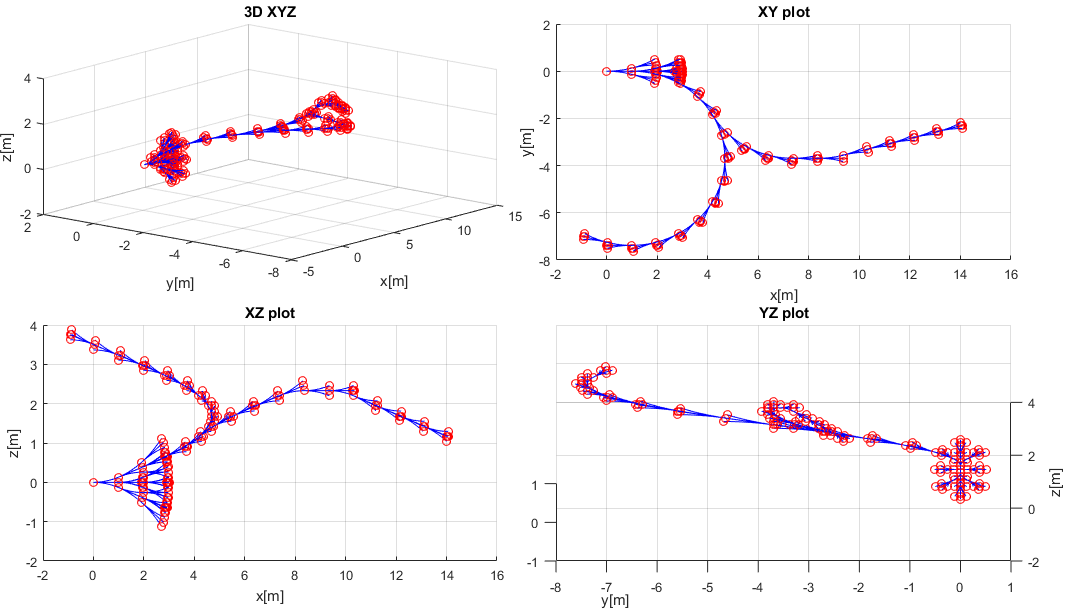
\includegraphics[width=0.9\linewidth]{\FIGDIR/RS001RapidExplorationTreeExampleShrink} 
    \caption{\emph{Rapid Exploration tree as result of \emph{Constrained trajectory expansion}}.}
    \label{fig:rapidExplorationTrajectoryTree}
\end{figure}

\paragraph{Rapid Exploration Tree} (fig. \ref{fig:rapidExplorationTrajectoryTree}) was selected, because it enables \emph{Movement Automaton Utilization} and \emph{Property Binding}. Similar approach was used for space exploration \cite{plaisant2002spacetree}. 

\paragraph{The example} (fig. \ref{fig:rapidExplorationTrajectoryTree}) shows a \emph{Rapid Exploration Tree} in \emph{Free Space} containing \emph{Waypoint Navigation Path} and \emph{Turn Away Path}. Both paths are starting in same \emph{Root Node} (red circle) which was expanded with simple \emph{Movement Automaton} (bunch of nodes originating from one node are showing way of expansion). The connection (blue line) between two nodes (red circles) represents \emph{Trajectory portion} for \emph{Executed Movement}.

\paragraph{Rapid Exploration Tree Node} will contain following information:
\begin{enumerate}
    \item \emph{Initial state} - root entry point, used in state evolution calculation.
    \item \emph{Trajectory (state evolution)} - trajectory passing through \emph{state space} in local coordinate frame of \emph{Avoidance Grid}.
    \item \emph{Buffer} (applied movements) - ordered list of \emph{executed movements} applied on \emph{initial state} to obtain \emph{state evolution}.
    \item \emph{Cost} - calculated for \emph{state evolution} based on \emph{predefined cost function}. 
    \item \emph{Footprint} - ordered set of \emph{passing cells} in \emph{Avoidance Grid}.
    \item \emph{Parent Node Reference} - tree reference for parent node, not in case of \emph{root node}.
    \item \emph{Other Bounded Properties} - value list of other properties, depending on \emph{Expansion Constraints} and \emph{Reachability} evaluation algorithm.
\end{enumerate}

\paragraph{Wave-front propagation of Rapid Exploration Tree} is given in (alg. \ref{alg:Wavefront Propagation}). 

The \emph{Avoidance Grid} have UAS with \emph{position $\in$ Initial State} at the \emph{origin}. The \emph{Grid Layer} is a column ordered set of cells with same \emph{Mean distance} from origin. \emph{Grid Layers} are indexed from origin starting with $1$, there is maximum of \emph{i $\ge$ 1} layers.

\paragraph{Step: Initialization} contains base structure preparation like follows:
\begin{enumerate}
    \item \emph{Avoidance Grid} - Space containing \emph{Reach set} (def. \ref{def:ContainedReducedReachSet}).
    \item \emph{Movement Automaton} - Used as \emph{Predictor}, consuming \emph{buffer} containing \emph{Movements} to generate $Trajectory(initialState,buffer)$.
    
    \item \emph{Reach Set} -  tree consisting from \emph{Wave-frontNodes} representing the end point of $Trajectory(initialState,buffer)$ where each \emph{Edge} represents \emph{one Movement application}. The root is set as node containing \emph{Initial State}.
\end{enumerate}

\noindent Function \emph{initializeReachSet(root,stack,grid,automaton)} will take the root and enforces \emph{full wavefornt propagation} to \emph{First Layer}.


\paragraph{Step: Wave-front Propagation} is forced propagation of trajectories from layer $i$ to layer $i+1$. The process goes as follows:
\begin{enumerate}
    \item \emph{Selection of Feasible candidates} - function \emph{[candidates,leftovers] = ExpansionConstraints.select(stack)} for working layer, row and cell selects \emph{feasible trajectory nodes} ordered by \emph{Cost function}. The \emph{Example of Cost Function} can be \emph{Trajectory Smoothness} (def. \ref{def:SmoothnessRatingForTrajectory}).
    
    \item \emph{Expansion of Candidates} - for each \emph{candidate} function \emph{candidate.expandNode (automaton)} is invoked. This function will expand \emph{Candidate Node structure} by appending \emph{Full Trajectory Tree Evolution} until each \emph{Leaf Trajectory} reaches \emph{Next Layer}. Simply put \emph{Par rent Node} \emph{Node(initialState, buffer, cost, footprint )} buffer is appended by movements until the next layer is reached.
    
    \item \emph{Leftovers purge} - function \emph{reachSet.purge(leftovers)} removes unexpanded \emph{Nodes} leading to cell, effectively  removing trajectories which does not  lead to \emph{next layer}.
    
    \item \emph{Append Reach Set} - function \emph{reachSet.append(leafs)} puts newly created \emph{Nodes (Trees)} into \emph{Reach Set} structure. The \emph{Wave-front Propagation} for one cell is finished.
\end{enumerate}

\paragraph{Step: After Layer Propagation Purge} is covered by function \emph{reachSet.purgeSame- Footprint()} which takes trajectories with same footprint and keeps some of them based on \emph{Selection criteria}, more in (sec. \ref{s:chaoticReachSet}, \ref{s:harmonicReachSet}). \emph{Pruning methods} over \emph{Large Decision Trees} are \emph{fast} and \emph{viable} \cite{mingers1989empirical}.

\begin{note}
    \emph{Reach Set} is usually computed \emph{Prior the Flight} for \emph{some Initial State} in \emph{Local Coordinate Frame} in \emph{right had coordinate frame} with $X^+$ used as \emph{main axis}.
\end{note}


\begin{algorithm}[H]
    \SetKwInOut{Input}{Input}\SetKwInOut{Output}{Output}
    \Input{Node(initialState,buffer=$\varnothing$,cost=0,footprint=$\varnothing$),
           AvoidanceGrid, ExpansionConstraints, MovementAutomaton(movementSet)
    }
    \Output{ReachSet(AvoidanceGrid)}
    \BlankLine
    \# Initialization Sequence\;
    grid=AvoidanceGrid, automaton=MovementAutomaton, root = Node\;
    reachSet = initializeReachSet(root,stack,grid,automaton)\;
    \BlankLine
    \# Main Expansion through, layers (i), rows (j), cells(k)\;
    \For{layer($1\dots i$) \emph{in} grid}{
        \For{row($1\dots j$ \emph{in} layer)}{
            \For{cell($1 \dots k$) \emph{in} row}{
                \BlankLine
                \# apply selection criteria \;
                [candidates,leftovers] = ExpansionConstraints.select(stack)\;
                \BlankLine
                \# collect expansions \;
                leafs = []\;
                \For{candidate \emph{in} Candidates}{
                    leafs= [leafs, candidate.expandNode(automaton)];
                }
                reachSet.purge(leftovers)\;
                reachSet.append(leafs)\;
            }
        }
        reachSet.purgeSameFootprint()\;
    }
    \caption{\emph{Wave-front propagation} of \emph{Rapid Exploration Tree} to form \emph{Reach Set}.}
    \label{alg:Wavefront Propagation}
\end{algorithm}






    	\subsection{Coverage-Maximizing Reach Set Approximation}\label{s:chaoticReachSet}

\paragraph{Summary:}

\paragraph{Motivation:} Design of calculation method for \emph{Reach Set Approximation} guarantying high \emph{Maneuverability}.

\paragraph{Background:}There is \emph{Coverage Ratio} property of \emph{Reach Set} (def. \ref{def:coverageRatio}). It has been shown that creating \emph{Reach Set} via \emph{greedy approach} is not feasible due to the \emph{Scaling Factor}.  \emph{Contracted Expansion} (sec. \ref{s:constrainedTrajectoryExpansion}) is enabling to apply selection criteria while building \emph{Reach Set} in given \emph{Cell}. 

The \emph{Cell} $cell_{i,j,k}$ has a center and walls from UAS viewpoint: a front wall, back wall (for $layer > 1$), a top wall, left wall, right wall, bottom wall. It is expected that trajectory leading close to one cell walls will continue to a different cell, increasing the chance to obtain more \emph{Unique Footprints}. 

\paragraph{Expansion Constraint Function Implementation} (alg. \ref{alg:ExpansionConstraintFunctionForChaoticReachSet}) is based on the simple principle: \emph{Select candidate Nodes which are  closest to outer walls of Cell, with a unique footprint}.

\paragraph{Tuning Parameters:} \emph{Proximity to Cell outer wall} gives good chances to break into other rows or columns in the \emph{Avoidance Grid}. \emph{Unique footprint} guarantees future \emph{Unique Footprint} after appending Trajectory by \emph{Movement application}. 
\begin{enumerate}
    \item \emph{Considered Footprint Length} - how much last cells in footprint should be considered in unique path track, minimal value 1, default value 3, maximal value $\infty$. If there is a need to generate non-redundant trajectories use $\infty$, it will consider full footprint.
    
    \item \emph{Spread Limit} - the upper limit of candidates which are going to be select for further expansion, minimal value 1, default value \emph{Count of unique Moves in Movement set}, maximal value $\infty$. If more than default values are selected, the algorithm will generate \emph{redundant trajectories}. If less is selected, then some trajectories are omitted, and \emph{Coverage Rate} decreases sharply. 
\end{enumerate}

\paragraph{Step: Initialization} initialization of \emph{candidate} array (return value), \emph{leftovers} array (return Value). Node array \emph{passing} is populated with \emph{Nodes} which represents \emph{end node of Trajectory}, and the tip of the  \emph{trajectory is constrained in the \emph{cell}$_{i,j,k}$}.

\paragraph{Step: Evaluate best trajectories with unique Footprints} following steps are executed:
\begin{enumerate}
    \item \emph{Best Performance Map} is created with a \emph{footprint} as a key set element to ensure footprint uniqueness.
    
    \item \emph{Wall distance} for the \emph{test node} is calculated as a closest trajectory portion distance to the \emph{top, bottom, left, right} wall of the $cell_{i,j,k}$
    
    \item The \emph{Footprint} for the \emph{test node} is created with the  maximal length given by \emph{Footprint Length} tuning parameter.
    
    \item \emph{Existence and Performance Test} is executed to ensure that the best performing node is selected. If there is no key entry in the \emph{Best Performance Map}, then a new entry for \emph{Test Node} is created. If there is a key entry, the performance of \emph{Old Node} and \emph{Test Node} is compared, and better is stored.
\end{enumerate}

\paragraph{Step: Select candidates} is executed on \emph{Best Performance Map} records using  \emph{Wall distance} as pivot parameter, ordering by closest proximity and limited by \emph{Search Limit} tuning parameter. The \emph{Leftovers} are difference set between \emph{Passing Nodes} and \emph{Candidate Nodes}. 


\begin{algorithm}[H]
    \SetKwInOut{Input}{Input}\SetKwInOut{Output}{Output}\SetKwInOut{TuningParameters}{Tuning Parameters}
    \Input{Node[] stack, Cell cell$_{i,j,k}$}
    \TuningParameters{int$^+$ footprintLength, int$^+$ spreadLimit}
    \Output{Node[] candidates, Node[] leftovers}
    
    \BlankLine
    \# Initialize structures\;
    Node[] candidates = [], Node[] leftovers=[]\;
    Node[] passing = cell$_{i,j,k}$.getFinishingTrajectories(stack)\;
    
    \BlankLine
    \# Select best performing trajectories with unique footprint\;
    Map$<$Footprint,Node$>$  bestPerformanceMap\;
    \For{Node test $\in$ passing}{
        wallDistance= test.minimalDistanceToWall(cell$_{i,j,k}$)]\;
        footPrint = test.getFootprint(lastCells = footprintLength)\;
        \eIf{bestPerformanceMap.contains(footPrint)}{
            old = bestPerformanceMap.getByKey(footprint)\;
            oldPerformance= old.minimalDistanceToWall(cell$_{i,j,k}$)\;
            \If{oldPerformance $>$ wallDistance}{
                bestPerformanceMap.setByKey(footprint,test)\;         
            }
        }{
            bestPerformanceMap.setByKey(footprint,test)\;
        }
    }
    
    \BlankLine
    \# Select best performing nodes up to \emph{spreadLimit} count\;
    candidates = bestPerformanceMap.select(count = spreadLimit).orderBy('wallDistance','Ascending')\;
    leftovers = passing - candidates\;
    \Return{[candidates,leftovers]}
    
    
    \caption{Expansion Constraint function for \emph{Coverage-Maximizing Reach Set Approximation}}
    \label{alg:ExpansionConstraintFunctionForChaoticReachSet}
\end{algorithm}


\paragraph{Example:} for \emph{Avoidance Grid} with \emph{Distance 10 m}, \emph{Layer count 10}, \emph{Horizontal range $[-45^\circ,+45^\circ]$}, \emph{Horizontal Cell Count 7}, \emph{Vertical range $[-30^\circ,+30^\circ]$}, and \emph{Vertical Cell Count 5}. Is given in (fig. \ref{fig:chaoticReachSetApproximation}). The UAS is at \emph{Back-side} of \emph{Figure} (initial state is at all \emph{Trajectory Origins}). The \emph{black dashed line} marks \emph{Avoidance Grid} space boundary. Each trajectory has its own color and ends at \emph{Front-side} of \emph{Avoidance Grid Boundary}.

\begin{figure}[H]
    \centering
    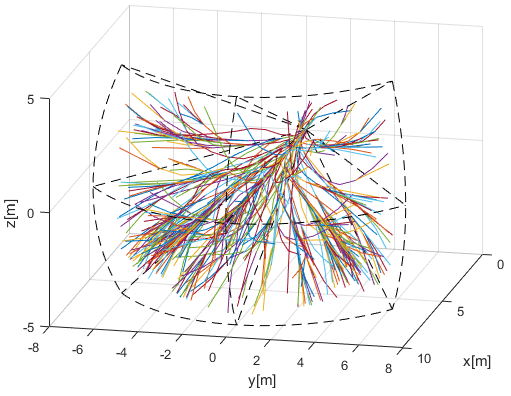
\includegraphics[width=0.7\linewidth]{\FIGDIR/RS002ChaoticReachSetEstimationMethod} 
    \caption{\emph{Coverage-Maximizing \emph{reach set} approximation}.}
    \label{fig:chaoticReachSetApproximation}
\end{figure}


\paragraph{Pros and Cons:} It can be seen from example (fig. \ref{fig:chaoticReachSetApproximation}) that \emph{Coverage-Maximizing Reach Set Approximation Method} (alg. \ref{alg:ExpansionConstraintFunctionForChaoticReachSet}) generates much \emph{turning} and \emph{shaky} \emph{trajectories}. 

\emph{High Coverage Ratio} ($\sim 0.9$) is provided while keeping \emph{medium node count}. The calculation complexity scales linearly with grid size. The \emph{upper limit of trajectories} is given as follow:

\begin{multline}
    countTrajectories(ReachSet) \le layerCellCount \times spreadLimit\\ \times size(Movements)
\end{multline}

\noindent The \emph{upper limit of nodes} is given as follow:
    
\begin{multline}
    countNodes(ReachSet) \le layerCount \times  layerCellCount  \\
    \times size(Movements) \times spreadLimit  
\end{multline}

\noindent The \emph{absence} of \emph{Smooth Trajectories} disqualifies \emph{Coverage Maximizing -RSA} to be used for \emph{Navigation}. This type of reach set is feasible for \emph{Avoidance} because it contains a variety of maneuvers.



    	\subsection{Turn-Minimizing Reach Set Approximation}\label{s:harmonicReachSet}

\paragraph{Motivation:} Imagine having an \emph{Avoidance Grid} like (fig. \ref{fig:LidarSpaceSegmentation}). There is a need of \emph{Reach Set Approximation} which will have \emph{Smooth Trajectories} (def. \ref{def:SmoothnessRatingForTrajectory}) going nearby $cell$ centers.

\paragraph{Background:} The \emph{Smoothness Rating for Trajectory} (def. \ref{def:SmoothnessRatingForTrajectory}) uses two distinct sets \emph{Smooth Movements} and \emph{Chaotic Movements} (eq. \ref{eq:ChaoticSmoothMovementSetDefinition}) which are defined for our \emph{Movement Automaton}  (sec. \ref{s:modelMAImplementation}) like follow:

\begin{equation}
    \begin{aligned}
    Smooth Movements &= \{Straight\} \\
    Chaotic Movements &= Movements - Smooth Movements\\
    \end{aligned}
\end{equation}

\emph{Smooth Movements} contains only \emph{Straight} movement, because others are considered as extreme turning movements. \emph{Smooth Movements} should contain only direct flight movements or slight heading correction. \emph{Chaotic Movements} set is supplement of \emph{Movement Automaton`s Movement Set}. 

The \emph{Avoidance Grid} (fig. \ref{fig:LidarSpaceSegmentation}) cell centers for fixed indexes $j_{fix}$, $k_{fix}$ are linearly aligned with \emph{initial state}. That means that  cell centers of cells $cell_{1,j_{fix},k_{fix}},\dots, cell_{i,j_{fix},k_{fix}}$, where $i$ is count of \emph{layers} lies on one line.  If the trajectory can achieve \emph{cell center} on some \emph{layer} only minor trajectory corrections are required to stay on given line. This type of trajectory gives us following advantages:
\begin{enumerate}
    \item\emph{Minimal steering at beginning} - the minimal steering is advantageous in \emph{Controlled Airspace} because is diminishing the amount of communication to \emph{UTM Service}.
    
    \item\emph{Additional safe space in Linear segment} - once the \emph{center of cell} is reached, \emph{Trajectory} sticks to line between cell centers. Each point on this line has \emph{maximal distance} to outer walls of cell. This gives us extra space given as minimum of distance between \emph{UAS position} and \emph{Outer cell walls}.
\end{enumerate}

\paragraph{Expansion Constraint Function Implementation} (alg. \ref{alg:ExpansionConstraintFunctionForHarmonicReachSet}) is based on simple principle: \emph{Select candidate Nodes  which are closest to Cell center, with unique footprint}.

\begin{note}
    \emph{Cell center} can be closely reached by \emph{smooth movement} from previous cell or \emph{chaotic movement} from neighbouring cell from current or previous layer. These trajectories are usually equivalent in \emph{Smoothness}.
\end{note}

\paragraph{Tuning Parameter:} \emph{Proximity to Cell Center} gives a good chance to keep trajectory smooth or \emph{smooth after one correction maneuver}. It has been mentioned that \emph{Cell Center} can be reached by various trajectories. In this method full footprint length is always considered, therefore only one tuning parameter can be offered:
\begin{enumerate}
    \item \emph{Spread Limit} - upper limit of candidates which are going to be selected for further expansion, minimal value 1, default value \emph{Count of unique Moves in Movement set}, maximal value $\infty$. If maximal value $\infty$ is selected, algorithm will generate skeleton of \emph{Reach Set} with full Coverage and with the smoothest \emph{Trajectories}.
\end{enumerate}

\paragraph{Step: Initialization} sets candidate \emph{Nodes} as empty set, leftover \emph{Nodes} as empty set. and selects all \emph{Nodes} from \emph{Stack} which represents  \emph{Finishing Trajectories} in working cell $cell_{i,j,k}$.

\begin{algorithm}[H]
\SetKwInOut{Input}{Input}\SetKwInOut{Output}{Output}\SetKwInOut{TuningParameters}{Tuning Parameters}
    \Input{Node[] stack, Cell cell$_{i,j,k}$}
    \TuningParameters{int$^+$ spreadLimit}
    \Output{Node[] candidates, Node[] leftovers}
    
    \BlankLine
    \# Initialize structures\;
    Node[] candidates = [], Node[] leftovers=[]\;
    Node[] passing = cell$_{i,j,k}$.getFinishingTrajectories(stack)\;
    
    \BlankLine
    \# Select unique smoothest trajectories\;
    Map$<$Buffer,Node$>$  bestPerformanceMap\;
    \For{Node test $\in$ passing}{
        centerDistance= test.getPerformance(cell$_{i,j,k}$)]\;
        footPrint = test.getFootprint()\;
        \eIf{bestPerformanceMap.contains(footPrint)}{
            old = bestPerformanceMap.getByKey(footprint)\;
            oldPerformance= old.getPerformance(cell$_{i,j,k}$)\;
            \If{oldPerformance $>$ centerDistance}{
                bestPerformanceMap.setByKey(footprint,test)\;         
            }
        }{
            bestPerformanceMap.setByKey(footprint,test)\;
        }
    }
    
    \BlankLine
    \# Select best performing nodes up to \emph{spreadLimit} count\;
    candidates = bestPerformanceMap.select(count = spreadLimit).orderBy('cellCenterDistance','Ascending')\;
    leftovers = passing - candidates\;
    \Return{[candidates,leftovers]}
    
    
    \caption{Expansion Constraint function for \emph{Harmonic Reach Set Approximation}}
    \label{alg:ExpansionConstraintFunctionForHarmonicReachSet}    
\end{algorithm}

\paragraph{Step: Evaluate smoothest trajectories with unique Footprints} is implemented as \emph{multi-criteria filtration}. 

\emph{First criterion} is \emph{distance to Cell Center} which is penalized by trajectory \emph{smoothness rate} implemented in method \emph{Node.getPerformance(Cell $cell_{i,j,k}$)} defined as follow.

\begin{equation}
    getPerformance(Node,Cell) = \frac{distance(Node.Trajectory,Cell.Center)}{SmoothnessRate(Node.Trajectory)}
\end{equation}

\noindent Distance of \emph{Trajectory} is \emph{enumerator}, because its considered as \emph{base value} and is defined in interval $[0,maximalWallDistance]$. The \emph{Smoothness Rate} is in denominator, because it is a penalization coefficient defined in interval $[0,1]$. 

\emph{Second criterion} is \emph{trajectory uniqueness} This is provided by \emph{Best Performance Map}, where best performing \emph{Node} belongs to one unique \emph{trajectory footprint}. The implementation is identical to \emph{chaotic reach set expansion} (alg. \ref{alg:ExpansionConstraintFunctionForChaoticReachSet}).

\paragraph{Step: Select candidates} is executed  on \emph{Best Performance Map} records using \emph{Penalized Cell Center Distance} as pivot parameter, ordered in ascending order and limited by \emph{Spread Limit} tuning parameter. The \emph{Leftovers} are difference set between \emph{Passing Nodes} and \emph{Candidate Nodes}.




\paragraph{Example:} for \emph{Avoidance Grid} with \emph{Distance 10 m}, \emph{Layer count 10}, \emph{Horizontal range $[-45^\circ,+45^\circ]$}, \emph{Horizontal Cell Count 7}, \emph{Vertical range $[-30^\circ,+30^\circ]$}, and \emph{Vertical Cell Count 5}. Is given in (fig. \ref{fig:harmonicReachSetApproximation}). The UAS is at \emph{Back-side} of \emph{Figure} (initial state is at all \emph{Trajectory Origins}). The \emph{black dashed line} marks \emph{Avoidance Grid} space boundary. Each trajectory has its own color and ends at \emph{Front-side} of \emph{Avoidance Grid Boundary}. The \emph{Spread Limit} in this case was set to $9$ which is \emph{Size of the Movement Set}.

\begin{note}
    Please note \emph{Trajectories} are organized in bundles going around \emph{Cell Centers smoothly}. Most of the steering maneuvers are executed at the \emph{beginning} of \emph{Avoidance Grid}.
\end{note}

\begin{figure}[H]
    \centering
    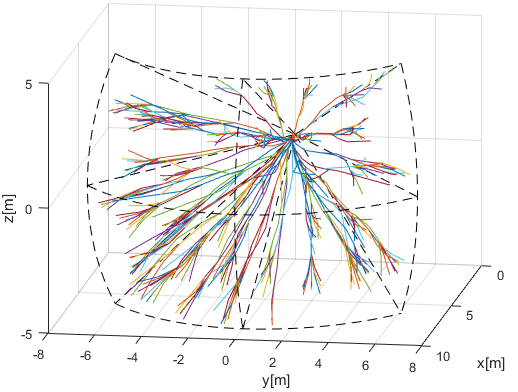
\includegraphics[width=0.7\linewidth]{\FIGDIR/RS003HarmonicReachSetEstimationMethod} 
    \caption{\emph{Harmonic \emph{reach set} approximation}.}
    \label{fig:harmonicReachSetApproximation}
\end{figure}

\paragraph{Pros and Cons:} It can bee seen from example (fig. \ref{fig:harmonicReachSetApproximation}) that \emph{Harmonic Reach Set Approximation Method} (alg. \ref{alg:ExpansionConstraintFunctionForHarmonicReachSet}) generates \emph{smooth evenly spread trajectories}.
    
High smoothness ratio ($\ge 0.9$) is provided, while keeping low node count for UAS systems. The calculation complexity scales linearly with grid size. The upper limit of trajectories is given as follow:

\begin{multline}
    countTrajectories(ReachSet) \le layerCellCount \times spreadLimit \\\times size(Movements)
\end{multline}

\noindent The \emph{upper limit of nodes} is given as follow:

\begin{equation}
    countNodes(ReachSet) \le layerCount \times layerCellCount \times spreadLimit
\end{equation}

\noindent Absence of \emph{High Coverage Ratio} disqualifies \emph{Harmonic Reach Set Approximation} to be used for \emph{Emergency Avoidance}. This type of \emph{Reach Set} is feasible for \emph{Open Space Navigation} or \emph{Controlled Airspace Navigation}. Its low turning rate in contained \emph{Trajectories} are desired for such tasks. 




    	\subsection{ACAS-X like Reach Set Approximation}\label{s:acasReachSet}
\paragraph{Motivation:} The implementation of \emph{ACAS-Xu} behavior in DAA system will  be mandatory for \emph{National Airspace System Integration} in United spaces \cite{shively2018uas}. 

Implementation of ACAS-Xu like behaviour increase usability of approach, if it can be achieved without major concept changes.


\paragraph{Background:} The \emph{ACAS-Xu} system on operational level has been described in \cite{marston2015acas}. The \emph{Policy for Collision Avoidance} proposal has been given in \cite{julian2016policy}.

Some behavioural patterns can be encoded into  \emph{Reach Set}. ACAS-Xu navigation part is basically \emph{Look-up table of Maneuvers for Allowed Separations}.
 
The \emph{Evasive Maneuver} selection process in ACAS-Xu is similar to our approach: \emph{Select most energy efficient maneuver in compliance with space-time constraints}. ACAS-Xu intruder model is similar to our \emph{Body Volume Intersection Model} (app. \ref{s:bodyvolumeIntersection}). The \emph{ACAS-Xu} defines following base separations:

\begin{enumerate}
    \item \emph{Horizontal} - movements on \emph{Horizontal Plane} in \emph{Global Coordinate System}.
    
    \item \emph{Vertical} - movements on \emph{Vertical Plane} in \emph{Global Coordinate System}.
    
\end{enumerate}

\noindent There are allowed custom separations which can be used, for further experimentation: 
\begin{enumerate}
    \item \emph{Slash} - movement on $+45^{\circ}$ \emph{Tilted Plane to Horizontal Plane} in \emph{Global Coordinate System}.
    
    \item \emph{Backslash} - movement on $-45^{\circ}$ \emph{Tilted Plane to Horizontal Plane} in \emph{Global Coordinate System}.
    
\end{enumerate}

\noindent For given \emph{Movement Automaton} implementation (sec. \ref{s:modelMAImplementation}) the separations are given as follow:

\begin{equation}\label{eq:implementedseparations}
    \begin{aligned}
        Horizontal & = \{Straight, Left, Right \}\\
        Vertical & = \{Straight, Up, Down\}\\
        Slash & = \{Straight, UpLeft, DownRight\}\\
        Backslash & = \{Straight, UpRight, DownLeft\}\\
    \end{aligned}
\end{equation}

\noindent For each $Node(\dots,buffer)$ and each \emph{separation} there is a evaluation function $isSeparation$ which decides, if \emph{Trajectory} defined by node buffer is made up only from \emph{Separation} movements.  The function $isSeparation(\dots)$ is defined like:

\begin{equation}\label{eq:isSeparationPredicate}
    isSeparation(buffer,separation) =
    \begin{cases}
        \begin{aligned}
            \forall & movement \in buffer,\\ & movement \in separation
        \end{aligned}&: true\\
        otherwise &: false
    \end{cases}
\end{equation}

\noindent Following \emph{Separation Modes} can be defined with given \emph{separations}:

\begin{enumerate}
    \item \emph{Horizontal} (ACAS-X defined mode) containing \emph{horizontal} separation. 
    
    \item \emph{Vertical} (ACAS-X defined mode) containing \emph{vertical} separation.
    
    \item \emph{Horizontal-Vertical} (ACAS-X defined mode) containing \emph{horizontal, vertical} separations.
    
    \item \emph{Full} (custom defined mode) containing all \emph{Separation Modes}.
    
\end{enumerate}

\begin{note}
    Every separation modes generates 2D trajectories set on \emph{Respective plane}. There is no need for \emph{Tuning parameters} for further \emph{Expansion Constraint}.    
\end{note}

\paragraph{Expansion Constraint Function Implementation} (alg. \ref{alg:ExpansionConstraintFunctionForACASLikeReachSet}) is based on simple principle:
\emph{Select only candidate Nodes which Trajectories have at least one desired Separation Mode}.

\paragraph{Step: Initialization} sets candidate \emph{Nodes} as empty set,  leftover \emph{Nodes} as empty set, and, select all nodes form \emph{stack} which represents \emph{Finishing Trajectories} in working $cell_{i,j,k}$,

\paragraph{Step: Candidate Selection Process} is evaluated for each \emph{test Node} from \emph{passing Node Set}. 

For each \emph{applicable separation}, given as input parameter \emph{separations}, The test function \emph{isSeparation} (eq. \ref{eq:isSeparationPredicate}) is applied:
\begin{enumerate}
    \item If \emph{test Node} trajectory belongs to at least one allowed separation it is added to candidates set.
    \item Else is added to \emph{Leftovers}.
\end{enumerate}

\begin{note}
    \emph{Separation sets} (eq. \ref{eq:implementedseparations}) are not \emph{exclusive sets} in \emph{Movement Automaton} domain. One \emph{Trajectory} contained by Node can belong to multiple \emph{Separations}.    
\end{note}

\begin{algorithm}[H]
\SetKwInOut{Input}{Input}\SetKwInOut{Output}{Output}\SetKwInOut{TuningParameters}{Tuning Parameters}
    \Input{Node[] stack, Cell cell$_{i,j,k}$, Separation[] separations}
    \TuningParameters{$None:\varnothing$}
    \Output{Node[] candidates, Node[] leftovers}
    
    \BlankLine
    \# Initialize structures\;
    Node[] candidates = [], Node[] leftovers=[]\;
    Node[] passing = cell$_{i,j,k}$.getFinishingTrajectories(stack)\;
    
    \BlankLine
    \# Select nodes containing trajectories with usable separations\;
    \For{Node test $\in$ passing}{
        \For{separation $\in$ separations}{
            \BlankLine
            \# Get separations for Node\;
            Separations[] nodeSeparations = test.getSeparations()\;
            \BlankLine
            \# If trajectory given by buffer is on Separation plane\;
            \If{isIn(isSeparation(test.buffer,separation)(\ref{eq:isSeparationPredicate})}{
                candidates.append(test)\;
            }
        }
        \BlankLine
        \# If there was no applicable separation, throw Node away\;
        \If{test $\not\in$ candidates}{
            leftovers.append(test)\;
        }
    }
    \BlankLine
    \# Return results\;
    \Return{[candidates,leftovers]}
    
    \caption{Expansion Constraint function for \emph{ACAS-like Reach Set Approximation}}
    \label{alg:ExpansionConstraintFunctionForACASLikeReachSet}    
\end{algorithm}

\paragraph{Example:} for \emph{Avoidance Grid} with \emph{Distance 10 m}, \emph{Layer count 10}, \emph{Horizontal range $[-45^\circ,+45^\circ]$}, \emph{Horizontal Cell Count 7}, \emph{Vertical range $[-30^\circ,+30^\circ]$}, and \emph{Vertical Cell Count 5}. Is given in (fig. \ref{fig:acasLikeReachSetVariousSeparationMode}). The UAS is at \emph{Back-side} of \emph{Figure} (initial state is at all \emph{Trajectory Origins}). The \emph{black dashed line} marks \emph{Avoidance Grid} space boundary. Each trajectory has its own color and ends at \emph{Front-side} of \emph{Avoidance Grid Boundary}.

\emph{Full} separation mode given in (fig. \ref{fig:acasLikeReachSetFull}). \emph{Horizontal-Vertical} separation mode, used in original \emph{ACAS-Xu} testing \cite{marston2015acas}, given in (fig. \ref{fig:acasLikeReachSetHorizontalVertical}). \emph{Horizontal} separation mode given in (fig. \ref{fig:acasLikeReachSetHorizontalOnly}) is usually used by planes. \emph{Vertical} separation mode given in (fig. \ref{fig:acasLikeReachSetVerticalOnly}) is usually used by copters.

\begin{figure}[H]
	\centering
    \begin{subfigure}{0.48\textwidth}
        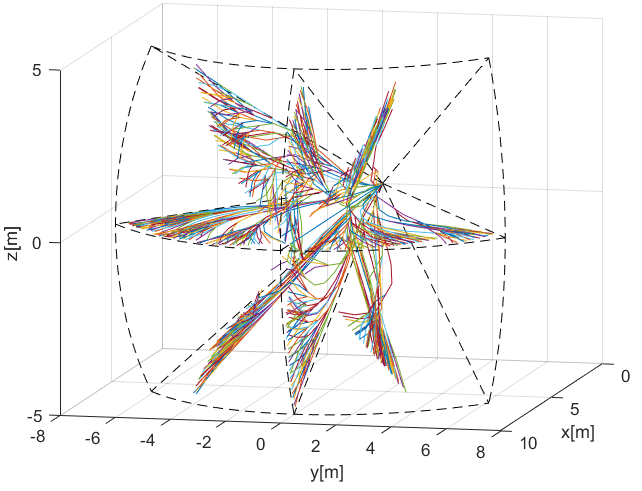
\includegraphics[width=0.9\linewidth]{\FIGDIR/RS005ACASLikeReachSetEstimationMethodFull}
        \caption{Full.}
        \label{fig:acasLikeReachSetFull}
    \end{subfigure}
    \begin{subfigure}{0.48\textwidth}
        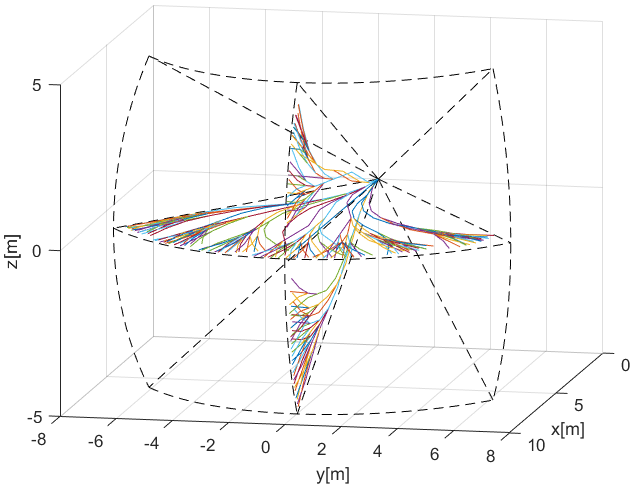
\includegraphics[width=0.9\linewidth]{\FIGDIR/RS006ACASLikeReachSetEstimationMethodHorizontalVertical} 
        \caption{Horizontal-Vertical.}
        \label{fig:acasLikeReachSetHorizontalVertical}
    \end{subfigure}
    \\
    \begin{subfigure}{0.48\textwidth}
        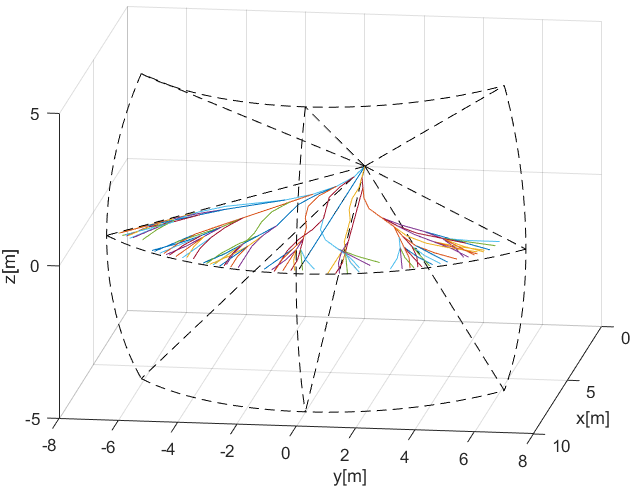
\includegraphics[width=0.9\linewidth]{\FIGDIR/RS008ACASLikeReachSetEstimationMethodHorizontal} 
        \caption{Horizontal.}
        \label{fig:acasLikeReachSetHorizontalOnly}
    \end{subfigure}
    \begin{subfigure}{0.48\textwidth}
        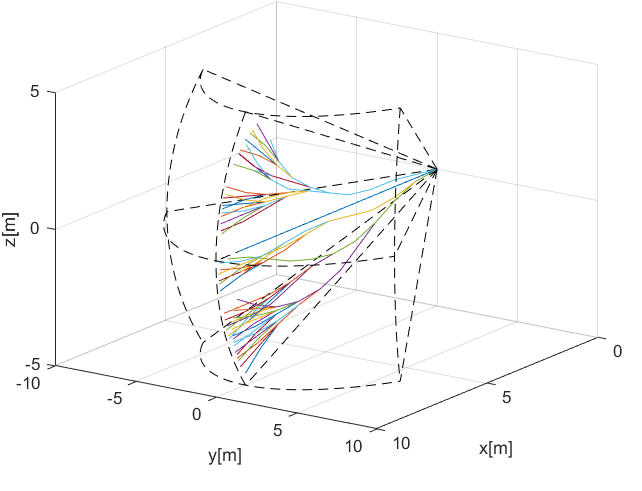
\includegraphics[width=0.9\linewidth]{\FIGDIR/RS009CASLikeReachSetEstimationMethodVertical} 
        \caption{Vertical.}
        \label{fig:acasLikeReachSetVerticalOnly}
    \end{subfigure}
    \caption{ACAS-X imitation \emph{reach set} approximation for various \emph{separation modes}. }
    \label{fig:acasLikeReachSetVariousSeparationMode}
\end{figure}

\paragraph{Pros and Cons:} It can be seen from examples (fig. \ref{fig:acasLikeReachSetVariousSeparationMode}) that \emph{ACAS-like Reach Set Approximation Method} (alg. \ref{alg:ExpansionConstraintFunctionForACASLikeReachSet}) generates full reach set for 2D plane located in 3D space. 

The \emph{Reach Set} contains trajectories with \emph{high coverage ratio} and \emph{high smoothness rating} for selected 2D separation plane. Overall performance compared to full 3D reach sets (sec. \ref{s:chaoticReachSet}, \ref{s:harmonicReachSet} \ref{s:combinedReachSet}) is poor. 

The \emph{node} and \emph{trajectory} count boundary was not implemented. It is common knowledge that \emph{2D} avoidance sets does not require scaling \cite{marston2015acas}. Otherwise trajectory footprint mechanism like in \emph{Harmonic Reach Set Approximation} (alg. \ref{alg:ExpansionConstraintFunctionForHarmonicReachSet}) can be introduced.

This reach set implements \emph{Planar-Separation} as native feature, it can be used for both \emph{navigation} and \emph{avoidance} tasks in \emph{Controlled Airspace}. For \emph{Non-controlled Airspace} there are far more superior \emph{Combined Reach Set} (sec. \ref{s:combinedReachSet}).

    	
\subsection{(R) Chaotic Reach set}\label{s:chaoticReachSet}

\paragraph{Motivation:} Design of calculation method for \emph{Reach Set Approximation} guarantying high \emph{Maneuverability}.

\paragraph{Background:}There is \emph{Coverage Ratio} property of \emph{Reach Set} (def. \ref{def:coverageRatio}). It has been shown that creating \emph{Reach Set} via \emph{greedy approach} is not feasible due the \emph{Scaling Factor}.  \emph{Contracted Expansion} (sec. \ref{s:constrainedTrajectoryExpansion}) is enabling to apply selection criteria while building \emph{Reach Set} in given \emph{Cell}. 

The \emph{Cell} $cell_{i,j,k}$ has a center and walls from UAS viewpoint: front wall , back wall (for $layer > 1$), top wall, left wall, right wall, bottom wall. It is expected that trajectory leading close to one cell walls will continue to different cell, increasing chance to obtain more \emph{Unique Footprints}. 

\paragraph{Expansion Constraint Function Implementation} (alg. \ref{alg:ExpansionConstraintFunctionForChaoticReachSet}) is based on simple principle: \emph{Select candidate Nodes which are  closest to outer walls of Cell, with unique footprint}.

\paragraph{Tuning Parameters}: \emph{Proximity to Cell outer wall} gives good chances to break into other rows or columns in \emph{Avoidance Grid}. \emph{Unique footprint} guarantees future \emph{Unique Footprint} after appending Trajectory by \emph{Movement application}. 
\begin{enumerate}
    \item \emph{Considered Footprint Length} - how much last cells in footprint should be considered in unique path track, minimal value 1, default value 3, maximal value $\infty$. If you want to generate non redundant trajectories use $\infty$, it will consider full footprint.
    
    \item \emph{Spread Limit} - upper limit of candidates which are going to be select for further expansion, minimal value 1, default value \emph{Count of unique Moves in Movement set}, maximal value $\infty$. If more than default values is selected the algorithm will generate \emph{redundant trajectories}. If less is selected then some trajectories are omitted and \emph{Coverage Rate} decreases sharply. 
\end{enumerate}


\paragraph{Step: Initialization} initialization of \emph{candidate} array (return value), \emph{leftovers} array (return Value). Node array \emph{passing} is populated with \emph{Nodes} which represents \emph{end node of Trajectory} and the tip of \emph{trajectory is constrained in \emph{cell}$_{i,j,k}$}.

\paragraph{Step: Evaluate best trajectories with unique Footprints} following steps are executed:
\begin{enumerate}
    \item \emph{Best Performance Map} is created with \emph{footprint} as key set element to ensure footprint uniqueness.
    \item \emph{Wall distance} for \emph{test node} is calculated as a closest trajectory portion distance to \emph{top, bottom, left, right} wall of cell $cell_{i,j,k}$
    \item \emph{Footprint} for \emph{test node} is created with maximal length given by \emph{Footprint Length} tuning parameter.
    \item \emph{Existence and Performance Test} is executed to ensure that best performing node is selected. If there is not key entry in the \emph{Best Performance Map}, then new entry for \emph{Test Node} is created. If there is key entry, the performance of \emph{Old Node} and \emph{Test Node} is compared and better is stored.
\end{enumerate}

\paragraph{Step: Select candidates} is executed on \emph{Best Performance Map} records using  \emph{Wall distance} as pivot parameter, ordering by closest proximity and limited by \emph{Search Limit} tuning parameter. The \emph{Leftovers} are difference set between \emph{Passing Nodes} and \emph{Candidate Nodes}. 

\begin{algorithm}[H]
    \SetKwInOut{Input}{Input}\SetKwInOut{Output}{Output}\SetKwInOut{TuningParameters}{Tuning Parameters}
    \Input{Node[] stack, Cell cell$_{i,j,k}$}
    \TuningParameters{int$^+$ footprintLength, int$^+$ spreadLimit}
    \Output{Node[] candidates, Node[] leftovers}
    
    \BlankLine
    \# Initialize structures\;
    Node[] candidates = [], Node[] leftovers=[]\;
    Node[] passing = cell$_{i,j,k}$.getFinishingTrajectories(stack)\;
    
    \BlankLine
    \# Select best performing trajectories with unique footprint\;
    Map$<$Footprint,Node$>$  bestPerformanceMap\;
    \For{Node test $\in$ passing}{
        wallDistance= test.minimalDistanceToWall(cell$_{i,j,k}$)]\;
        footPrint = test.getFootprint(lastCells = footprintLength)\;
        \eIf{bestPerformanceMap.contains(footPrint)}{
            old = bestPerformanceMap.getByKey(footprint)\;
            oldPerformance= old.minimalDistanceToWall(cell$_{i,j,k}$)\;
            \If{oldPerformance $>$ wallDistance}{
                bestPerformanceMap.setByKey(footprint,test)\;         
            }
        }{
            bestPerformanceMap.setByKey(footprint,test)\;
        }
    }
    
    \BlankLine
    \# Select best performing nodes up to \emph{spreadLimit} count\;
    candidates = bestPerformanceMap.select(count = spreadLimit).orderBy('wallDistance','Ascending')\;
    leftovers = passing - candidates\;
    \Return{[candidates,leftovers]}
    
    
    \caption{Expansion Constraint function for \emph{Chaotic Reach Set Approximation}}
    \label{alg:ExpansionConstraintFunctionForChaoticReachSet}
\end{algorithm}

\paragraph{Example:} for \emph{Avoidance Grid} with \emph{Distance 10 m}, \emph{Layer count 10}, \emph{Horizontal range $[-45^\circ,+45^\circ]$}, \emph{Horizontal Cell Count 7}, \emph{Vertical range $[-30^\circ,+30^\circ]$}, and \emph{Vertical Cell Count 5}. Is given in (fig. \ref{fig:chaoticReachSetApproximation}). The UAS is at \emph{Back-side} of \emph{Figure} (initial state is at all \emph{Trajectory Origins}). The \emph{black dashed line} marks \emph{Avoidance Grid} space boundary. Each trajectory has its own color and ends at \emph{Front-side} of \emph{Avoidance Grid Boundary}.


\begin{figure}[H]
    \centering
    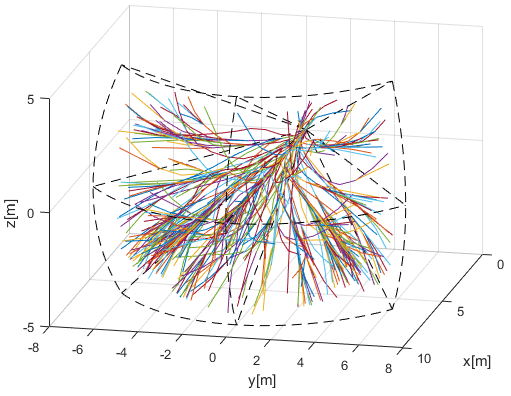
\includegraphics[width=0.7\linewidth]{\FIGDIR/RS002ChaoticReachSetEstimationMethod} 
    \caption{\emph{Chaotic \emph{reach set} approximation}.}
    \label{fig:chaoticReachSetApproximation}
\end{figure}

\paragraph{Pros and Cons:} It can be seen from example (fig. \ref{fig:chaoticReachSetApproximation}) that \emph{Chaotic Reach Set Approximation Method} (alg. \ref{alg:ExpansionConstraintFunctionForChaoticReachSet}) generates a lot of \emph{turning} and \emph{shaky} \emph{trajectories}. 

\emph{High Coverage Ratio} ($\sim 0.9$) is provided, while keeping \emph{medium node count}. The calculation complexity scales linearly with grid size. The \emph{upper limit of trajectories} is given as follow:

\begin{multline}
    countTrajectories(ReachSet) \le layerCellCount \times spreadLimit\\ \times size(Movements)
\end{multline}

\noindent The \emph{upper limit of nodes} is given as follow:
    
\begin{multline}
    countNodes(ReachSet) \le layerCount \times  layerCellCount  \\
    \times size(Movements) \times spreadLimit  
\end{multline}

\noindent\emph{Absence} of \emph{Smooth Trajectories} disqualifies \emph{Chaotic Reach Set Approximation} to be used for \emph{Navigation}. This type of reach set is feasible for \emph{Avoidance}, because it contains variety of maneuvers.


\subsection{(R) Harmonic Reach set}\label{s:harmonicReachSet}

\paragraph{Motivation:} Imagine having an \emph{Avoidance Grid} like (fig. \ref{fig:LidarSpaceSegmentation}). There is a need of \emph{Reach Set Approximation} which will have \emph{Smooth Trajectories} (def. \ref{def:SmoothnessRatingForTrajectory}) going nearby $cell$ centers.

\paragraph{Background:} The \emph{Smoothness Rating for Trajectory} (def. \ref{def:SmoothnessRatingForTrajectory}) uses two distinct sets \emph{Smooth Movements} and \emph{Chaotic Movements} (eq. \ref{eq:ChaoticSmoothMovementSetDefinition}) which are defined for our \emph{Movement Automaton}  (sec. \ref{s:modelMAImplementation}) like follow:

\begin{equation}
    \begin{aligned}
    Smooth Movements &= \{Straight\} \\
    Chaotic Movements &= Movements - Smooth Movements\\
    \end{aligned}
\end{equation}

\emph{Smooth Movements} contains only \emph{Straight} movement, because others are considered as extreme turning movements. \emph{Smooth Movements} should contain only direct flight movements or slight heading correction. \emph{Chaotic Movements} set is supplement of \emph{Movement Automaton`s Movement Set}. 

The \emph{Avoidance Grid} (fig. \ref{fig:LidarSpaceSegmentation}) cell centers for fixed indexes $j_{fix}$, $k_{fix}$ are linearly aligned with \emph{initial state}. That means that  cell centers of cells $cell_{1,j_{fix},k_{fix}},\dots, cell_{i,j_{fix},k_{fix}}$, where $i$ is count of \emph{layers} lies on one line.  If the trajectory can achieve \emph{cell center} on some \emph{layer} only minor trajectory corrections are required to stay on given line. This type of trajectory gives us following advantages:
\begin{enumerate}
    \item\emph{Minimal steering at beginning} - the minimal steering is advantageous in \emph{Controlled Airspace} because is diminishing the amount of communication to \emph{UTM Service}.
    
    \item\emph{Additional safe space in Linear segment} - once the \emph{center of cell} is reached, \emph{Trajectory} sticks to line between cell centers. Each point on this line has \emph{maximal distance} to outer walls of cell. This gives us extra space given as minimum of distance between \emph{UAS position} and \emph{Outer cell walls}.
\end{enumerate}

\paragraph{Expansion Constraint Function Implementation} (alg. \ref{alg:ExpansionConstraintFunctionForHarmonicReachSet}) is based on simple principle: \emph{Select candidate Nodes  which are closest to Cell center, with unique footprint}.

\begin{note}
    \emph{Cell center} can be closely reached by \emph{smooth movement} from previous cell or \emph{chaotic movement} from neighbouring cell from current or previous layer. These trajectories are usually equivalent in \emph{Smoothness}.
\end{note}

\paragraph{Tuning Parameter:} \emph{Proximity to Cell Center} gives a good chance to keep trajectory smooth or \emph{smooth after one correction maneuver}. It has been mentioned that \emph{Cell Center} can be reached by various trajectories. In this method full footprint length is always considered, therefore only one tuning parameter can be offered:
\begin{enumerate}
    \item \emph{Spread Limit} - upper limit of candidates which are going to be selected for further expansion, minimal value 1, default value \emph{Count of unique Moves in Movement set}, maximal value $\infty$. If maximal value $\infty$ is selected, algorithm will generate skeleton of \emph{Reach Set} with full Coverage and with the smoothest \emph{Trajectories}.
\end{enumerate}

\paragraph{Step: Initialization} sets candidate \emph{Nodes} as empty set, leftover \emph{Nodes} as empty set. and selects all \emph{Nodes} from \emph{Stack} which represents  \emph{Finishing Trajectories} in working cell $cell_{i,j,k}$.

\paragraph{Step: Evaluate smoothest trajectories with unique Footprints} is implemented as \emph{multi-criteria filtration}. 

\emph{First criterion} is \emph{distance to Cell Center} which is penalized by trajectory \emph{smoothness rate} implemented in method \emph{Node.getPerformance(Cell $cell_{i,j,k}$)} defined as follow.

\begin{equation}
    getPerformance(Node,Cell) = \frac{distance(Node.Trajectory,Cell.Center)}{SmoothnessRate(Node.Trajectory)}
\end{equation}

\noindent Distance of \emph{Trajectory} is \emph{enumerator}, because its considered as \emph{base value} and is defined in interval $[0,maximalWallDistance]$. The \emph{Smoothness Rate} is in denominator, because it is a penalization coefficient defined in interval $[0,1]$. 

\emph{Second criterion} is \emph{trajectory uniqueness} This is provided by \emph{Best Performance Map}, where best performing \emph{Node} belongs to one unique \emph{trajectory footprint}. The implementation is identical to \emph{chaotic reach set expansion} (alg. \ref{alg:ExpansionConstraintFunctionForChaoticReachSet}).

\paragraph{Step: Select candidates} is executed  on \emph{Best Performance Map} records using \emph{Penalized Cell Center Distance} as pivot parameter, ordered in ascending order and limited by \emph{Spread Limit} tuning parameter. The \emph{Leftovers} are difference set between \emph{Passing Nodes} and \emph{Candidate Nodes}.

\begin{algorithm}[H]
\SetKwInOut{Input}{Input}\SetKwInOut{Output}{Output}\SetKwInOut{TuningParameters}{Tuning Parameters}
    \Input{Node[] stack, Cell cell$_{i,j,k}$}
    \TuningParameters{int$^+$ spreadLimit}
    \Output{Node[] candidates, Node[] leftovers}
    
    \BlankLine
    \# Initialize structures\;
    Node[] candidates = [], Node[] leftovers=[]\;
    Node[] passing = cell$_{i,j,k}$.getFinishingTrajectories(stack)\;
    
    \BlankLine
    \# Select unique smoothest trajectories\;
    Map$<$Buffer,Node$>$  bestPerformanceMap\;
    \For{Node test $\in$ passing}{
        centerDistance= test.getPerformance(cell$_{i,j,k}$)]\;
        footPrint = test.getFootprint()\;
        \eIf{bestPerformanceMap.contains(footPrint)}{
            old = bestPerformanceMap.getByKey(footprint)\;
            oldPerformance= old.getPerformance(cell$_{i,j,k}$)\;
            \If{oldPerformance $>$ centerDistance}{
                bestPerformanceMap.setByKey(footprint,test)\;         
            }
        }{
            bestPerformanceMap.setByKey(footprint,test)\;
        }
    }
    
    \BlankLine
    \# Select best performing nodes up to \emph{spreadLimit} count\;
    candidates = bestPerformanceMap.select(count = spreadLimit).orderBy('cellCenterDistance','Ascending')\;
    leftovers = passing - candidates\;
    \Return{[candidates,leftovers]}
    
    
    \caption{Expansion Constraint function for \emph{Harmonic Reach Set Approximation}}
    \label{alg:ExpansionConstraintFunctionForHarmonicReachSet}    
\end{algorithm}


\paragraph{Example:} for \emph{Avoidance Grid} with \emph{Distance 10 m}, \emph{Layer count 10}, \emph{Horizontal range $[-45^\circ,+45^\circ]$}, \emph{Horizontal Cell Count 7}, \emph{Vertical range $[-30^\circ,+30^\circ]$}, and \emph{Vertical Cell Count 5}. Is given in (fig. \ref{fig:harmonicReachSetApproximation}). The UAS is at \emph{Back-side} of \emph{Figure} (initial state is at all \emph{Trajectory Origins}). The \emph{black dashed line} marks \emph{Avoidance Grid} space boundary. Each trajectory has its own color and ends at \emph{Front-side} of \emph{Avoidance Grid Boundary}. The \emph{Spread Limit} in this case was set to $9$ which is \emph{Size of the Movement Set}.

\begin{note}
    Please note \emph{Trajectories} are organized in bundles going around \emph{Cell Centers smoothly}. Most of the steering maneuvers are executed at the \emph{beginning} of \emph{Avoidance Grid}.
\end{note}

\begin{figure}[H]
    \centering
    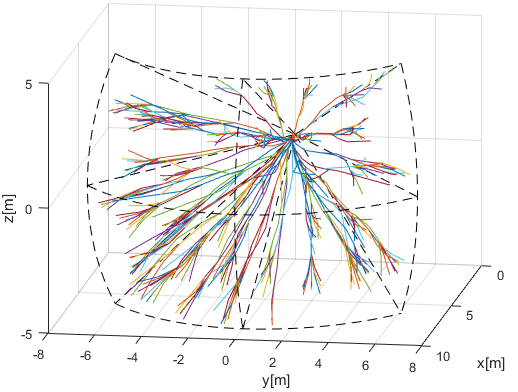
\includegraphics[width=0.7\linewidth]{\FIGDIR/RS003HarmonicReachSetEstimationMethod} 
    \caption{\emph{Harmonic \emph{reach set} approximation}.}
    \label{fig:harmonicReachSetApproximation}
\end{figure}

\paragraph{Pros and Cons:} It can bee seen from example (fig. \ref{fig:harmonicReachSetApproximation}) that \emph{Harmonic Reach Set Approximation Method} (alg. \ref{alg:ExpansionConstraintFunctionForHarmonicReachSet}) generates \emph{smooth evenly spread trajectories}.
    
High smoothness ratio ($\ge 0.9$) is provided, while keeping low node count for UAS systems. The calculation complexity scales linearly with grid size. The upper limit of trajectories is given as follow:

\begin{multline}
    countTrajectories(ReachSet) \le layerCellCount \times spreadLimit \\\times size(Movements)
\end{multline}

\noindent The \emph{upper limit of nodes} is given as follow:

\begin{equation}
    countNodes(ReachSet) \le layerCount \times layerCellCount \times spreadLimit
\end{equation}

\noindent Absence of \emph{High Coverage Ratio} disqualifies \emph{Harmonic Reach Set Approximation} to be used for \emph{Emergency Avoidance}. This type of \emph{Reach Set} is feasible for \emph{Open Space Navigation} or \emph{Controlled Airspace Navigation}. Its low turning rate in contained \emph{Trajectories} are desired for such tasks. 



\subsection{(R) Combined Reach set}\label{s:combinedReachSet}
\paragraph{Motivation:} Harmonic reach set (sec. \ref{s:harmonicReachSet}) is \emph{efficient} for \emph{Navigation in \emph{Controlled Airspace}}. Chaotic reach set (sec. \ref{s:chaoticReachSet}) is good for \emph{Emergency avoidance}. The need to differentiation between \emph{Navigation} and \emph{Emergency Avoidance} mode is necessary in \emph{Controlled Airspace}. but not in \emph{Non-controlled Airspace}. The combination of \emph{Harmonic} and \emph{Chaotic} reach sets is obvious solution. 

\emph{Automatic mode switch} can be provided by combination of \emph{Navigation Reach Set} and \emph{Avoidance Reach Set} with elevated cost function. Overall having a method to merge multiple trees would be beneficial.

\paragraph{Background:} If two \emph{Reach Set Approximation} were calculated for same \emph{Avoidance Grid} and \emph{Initial State}, using same \emph{Movement Automaton} and \emph{UAS model} are possible to merge. 

The \emph{Reach Set Approximation} is \emph{tree} with \emph{Root Node} in \emph{initail state} with movement buffer = $\varnothing$. The \emph{movement buffer} in each node can be used as \emph{route trace} during merging procedure. The example two reach set merge can be given as follow, where only \emph{latest} applied movement is taken into account.

\begin{equation}\label{eq:mergeTreeFunctionExample}
    \left[
    \begin{aligned}
    \texttt{Fi}&\texttt{rst Reach Set}\\
        &\varnothing \to 
            \left<
                \begin{aligned}
                    &left \to \left<
                                \begin{aligned}
                                    &left\\
                                    &right
                                \end{aligned}
                              \right.\\
                    &\varnothing\\
                \end{aligned}
             \right.\\ 
    \texttt{Se}&\texttt{cond Reach Set}\\
        &\varnothing \to 
            \left<
                \begin{aligned}
                    & \varnothing \\
                    & right \to \left< 
                                    \begin{aligned}
                                        &left\\
                                        &right
                                    \end{aligned}
                                \right.\\
                \end{aligned}
            \right.\\
    \end{aligned}
    \right]
    \to
    \left[
    \begin{aligned}
    \texttt{Co}&\texttt{mbined Reach Set}\\
    &\varnothing\to
        \left< 
            \begin{aligned}
                &left &\to   \left< 
                                \begin{aligned}
                                    &left\\
                                    &right
                                \end{aligned}    
                            \right.\\
                &right &\to   \left< 
                                \begin{aligned}
                                    &left\\
                                    &right
                                \end{aligned}    
                            \right.\\
            \end{aligned}    
        \right.
    \end{aligned}
    \right]
\end{equation}

\emph{First Reach Set} contains two trajectories given by buffers \emph{\{left,left\}} and \emph{\{left,right\}}. \emph{Second Reach Set} contains two trajectories given by buffers \emph{\{right,left\}} and \emph{\{right,right\}}. The \emph{Combined Reach Set} contains all four trajectories.

\begin{note}
    The combined tree \cite{o1996log} does not need to have combined amount of original \emph{Reach Sets} trajectories. There can be \emph{Duplicity} which means that any bounded property like \emph{Cost} must be \emph{calculated} again.
\end{note}

\paragraph{Combined Reach Set Calculation Function} (alg. \ref{alg:ReachSetMerge}) is implemented as function $Node combinedReachSet(\dots)$ which takes root Node with \emph{initial State}, \emph{Avoidance Grid} and respective parameters for each calculation method. \emph{Harmonic spread} for \emph{Harmonic Reach set calculation} and \emph{Chaotic Spread}, \emph{Footprint Length} for \emph{Chaotic Reach set calculation}.

\emph{Separate Reach Sets} are calculated using \emph{Wave-front propagation} (alg. \ref{alg:Wavefront Propagation}) using respective \emph{Constrained Expansion} functions for \emph{Harmonic} (alg. \ref{alg:ExpansionConstraintFunctionForHarmonicReachSet}) and \emph{Chaotic} (alg. \ref{alg:ExpansionConstraintFunctionForChaoticReachSet}) reach sets.

\emph{Combined Reach Set} is created using \emph{Node mergeTree($\dots$)} function. Because different cost function or \emph{Bounded Parameters Calculation} may be applied on \emph{Original Reach Sets}.

\emph{Cost} for \emph{each node} needs to be recalculated due to original reach sets disparity. Function \emph{combined.applyCostFunction()} will recalculate the new cost for each node. 

The Goal is to have penalization for \emph{Chaotic behaviour}, implementation of \emph{Automatic Mode Switch} can be done like follows:
\begin{enumerate}
    \item \emph{Calculate Normal Cost} for Node $Cost(Node)$ for associated trajectory:\\ $Cost(Node.Trajectory)$.
    \item \emph{Calculate Penalization for \emph{Chaotic Behaviour}}, calculate \emph{Smoothness Rating for Trajectory} (def. \ref{def:SmoothnessRatingForTrajectory}) in interval $[0,1]$, introduce penalization with base $100 \%$.
\end{enumerate}

The final $Cost(Node)$ function is applied on each \emph{Combined Reach Set Node} and look like follows:

\begin{multline}
    Cost(Node) = Cost(Node.Trajectory) \times\dots\\\dots\times \left(1+ \left(1-SmoothnessRate(N ode.T rajectory)\right)\right)
\end{multline}

\paragraph{Merge Tree Function} $mergeTree(\dots)$ implements \emph{Outer Join} operation on two trees. Example was given in (eq. \ref{eq:mergeTreeFunctionExample}).
Function is applied on \emph{root Node} iterating over \emph{Movements in Movement Set}, because \emph{Movement is pivot}.

\begin{algorithm}[H]
    \SetKwProg{Fn}{}{}{}\SetKwFunction{FRecurs}{Node mergeTree}
    \SetKwProg{Fn}{}{}{}\SetKwFunction{FMain}{Node combinedReachSet}
    
    \BlankLine
    \# Tree merge function\;
    \Fn(){\FRecurs{Node firstNode, Node secondNode}}{
        \BlankLine
        \# Try to copy reference node or return null\;
        Node referenceNode = (firstNode?:(secondNode?: return null))\;
        Node merged =  new Node(referenceNode)\;
        merged.leafs= []\;
        \BlankLine
        \# Try to fetch movement nodes if exist in any sub tree\;
        \For{movement $\in$ Movements}{
            firstLeaf = firstNode.getLeafFor(movement)\;
            secondLeaf = secondNode.getLeafFor(movement)\;
            newLeaf = mergeTree(firstLeaf,secondLeaf)\;
            \If{newLeaf $\sim = $ null}{
                merged.leafs.append(newLeaf)\;
            }
        }
        \Return{merged}
    }{}
    
    \BlankLine
    \# Combined Reach Set calculation function\;
    \Fn(){\FMain{Node root, AvoidanceGrid grid,int$^+$ chaoticSpread, int$^+$ harmonicSpread, int$^+$ footprintLength}}{
        Node chaotic = chaoticReachSet(root,grid, footprintLength,chaoticSpread)\;
        Node harmonic = harmonicReachSet(root,grid, harmonicSpread)\;
        Node combined = mergeTree(chaotic,harmonic)\;
        combined.applyCostFunction()\;
        \Return{combined}
    }

    
    \caption{Reach Set Merge Function and Combined Reach Set calculation}
    \label{alg:ReachSetMerge}
\end{algorithm}

\paragraph{Example:} for \emph{Avoidance Grid} with \emph{Distance 10 m}, \emph{Layer count 10}, \emph{Horizontal range $[-45^\circ,+45^\circ]$}, \emph{Horizontal Cell Count 7}, \emph{Vertical range $[-30^\circ,+30^\circ]$}, and \emph{Vertical Cell Count 5}. Is given in (fig. \ref{fig:combinedReachSetApproximation}). The UAS is at \emph{Back-side} of \emph{Figure} (initial state is at all \emph{Trajectory Origins}). The \emph{black dashed line} marks \emph{Avoidance Grid} space boundary. Each trajectory has its own color and ends at \emph{Front-side} of \emph{Avoidance Grid Boundary}. The \emph{Chaotic Spread} was set to 8, \emph{Footprint Length} to 3 and \emph{Harmonic Spread} to 1.

\begin{note}
    Notice there are typical trajectories from both \emph{Harmonic} (fig. \ref{fig:harmonicReachSetApproximation}) and \emph{Chaotic} (fig. \ref{fig:chaoticReachSetApproximation}) \emph{Reach Set Approximations}.
\end{note}

\begin{figure}[H]
    \centering
    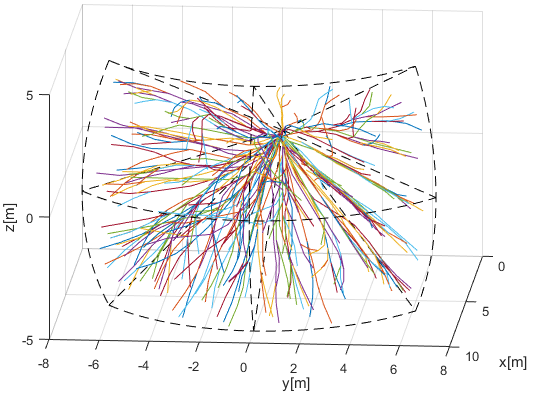
\includegraphics[width=0.7\linewidth]{\FIGDIR/RS004CombinedReachSetEstimationMethod} 
    \caption{\emph{Combined \emph{reach set} approximation}.}
    \label{fig:combinedReachSetApproximation}
\end{figure}


\paragraph{Pros and Cons:} It can bee seen from example (fig. \ref{fig:combinedReachSetApproximation}) that \emph{Combined Reach Set Approximation} (alg. \ref{alg:ReachSetMerge}) contains both types of maneuvers. \emph{Cheaper Smooth} for navigation and \emph{More Expensive Chaotic} for \emph{Emergency Avoidance}. The upper limit of trajectories is given as follow:

\begin{multline}
    countTrajectories(ReachSet) \le countTrajectories(Chaotic) \\+ countTrajectories(Harmonic)
\end{multline}

\noindent The \emph{upper limit of nodes} is given as follow:

\begin{equation}
    countNodes(ReachSet) \le countNodes(Chaotic)+ countNodes(Harmonic)
\end{equation}

\noindent \emph{Harmonic Reach Set} is ideal for \emph{Non-controlled Airspace} missions, because it contains \emph{Automatic Mode Switch} between \emph{Navigation} and \emph{Emergency Avoidance}.


\subsection{(R) ACAS-X like Reach set}\label{s:acasReachSet}
\paragraph{Motivation:} The implementation of \emph{ACAS-Xu} behavior in DAA system will  be mandatory for \emph{National Airspace System Integration} in United spaces \cite{shively2018uas}. 

Implementation of ACAS-Xu like behaviour increase usability of approach, if it can be achieved without major concept changes.


\paragraph{Background:} The \emph{ACAS-Xu} system on operational level has been described in \cite{marston2015acas}. The \emph{Policy for Collision Avoidance} proposal has been given in \cite{julian2016policy}.

Some behavioural patterns can be encoded into  \emph{Reach Set}. ACAS-Xu navigation part is basically \emph{Look-up table of Maneuvers for Allowed Separations}.
 
The \emph{Evasive Maneuver} selection process in ACAS-Xu is similar to our approach: \emph{Select most energy efficient maneuver in compliance with space-time constraints}. ACAS-Xu intruder model is similar to our \emph{Body Volume Intersection Model} (sec. \ref{s:bodyvolumeIntersection}). The \emph{ACAS-Xu} defines following base separations:

\begin{enumerate}
    \item \emph{Horizontal} - movements on \emph{Horizontal Plane} in \emph{Global Coordinate System}.
    
    \item \emph{Vertical} - movements on \emph{Vertical Plane} in \emph{Global Coordinate System}.
    
\end{enumerate}

\noindent There are allowed custom separations which can be used, for further experimentation: 
\begin{enumerate}
    \item \emph{Slash} - movement on $+45^{\circ}$ \emph{Tilted Plane to Horizontal Plane} in \emph{Global Coordinate System}.
    
    \item \emph{Backslash} - movement on $-45^{\circ}$ \emph{Tilted Plane to Horizontal Plane} in \emph{Global Coordinate System}.
    
\end{enumerate}

\noindent For given \emph{Movement Automaton} implementation (sec. \ref{s:modelMAImplementation}) the separations are given as follow:

\begin{equation}\label{eq:implementedseparations}
    \begin{aligned}
        Horizontal & = \{Straight, Left, Right \}\\
        Vertical & = \{Straight, Up, Down\}\\
        Slash & = \{Straight, UpLeft, DownRight\}\\
        Backslash & = \{Straight, UpRight, DownLeft\}\\
    \end{aligned}
\end{equation}

\noindent For each $Node(\dots,buffer)$ and each \emph{separation} there is a evaluation function $isSeparation$ which decides, if \emph{Trajectory} defined by node buffer is made up only from \emph{Separation} movements.  The function $isSeparation(\dots)$ is defined like:

\begin{equation}\label{eq:isSeparationPredicate}
    isSeparation(buffer,separation) =
    \begin{cases}
        \begin{aligned}
            \forall & movement \in buffer,\\ & movement \in separation
        \end{aligned}&: true\\
        otherwise &: false
    \end{cases}
\end{equation}

Following \emph{Separation Modes} can be defined with given \emph{separations}:

\begin{enumerate}
    \item \emph{Horizontal} (ACAS-X defined mode) containing \emph{horizontal} separation. 
    
    \item \emph{Vertical} (ACAS-X defined mode) containing \emph{vertical} separation.
    
    \item \emph{Horizontal-Vertical} (ACAS-X defined mode) containing \emph{horizontal, vertical} separations.
    
    \item \emph{Full} (custom defined mode) containing all \emph{Separation Modes}.
    
\end{enumerate}

\begin{note}
    Every separation modes generates 2D trajectories set on \emph{Respective plane}. There is no need for \emph{Tuning parameters} for further \emph{Expansion Constraint}.    
\end{note}

\paragraph{Expansion Constraint Function Implementation} (alg. \ref{alg:ExpansionConstraintFunctionForACASLikeReachSet}) is based on simple principle:
\emph{Select only candidate Nodes which Trajectories have at least one desired Separation Mode}.

\paragraph{Step: Initialization} sets candidate \emph{Nodes} as empty set,  leftover \emph{Nodes} as empty set, and, select all nodes form \emph{stack} which represents \emph{Finishing Trajectories} in working $cell_{i,j,k}$,

\paragraph{Step: Candidate Selection Process} is evaluated for each \emph{test Node} from \emph{passing Node Set}. 

For each \emph{applicable separation}, given as input parameter \emph{separations}, The test function \emph{isSeparation} (eq. \ref{eq:isSeparationPredicate}) is applied:
\begin{enumerate}
    \item If \emph{test Node} trajectory belongs to at least one allowed separation it is added to candidates set.
    \item Else is added to \emph{Leftovers}.
\end{enumerate}

\begin{note}
    \emph{Separation sets} (eq. \ref{eq:implementedseparations}) are not \emph{exclusive sets} in \emph{Movement Automaton} domain. One \emph{Trajectory} contained by Node can belong to multiple \emph{Separations}.    
\end{note}

\begin{algorithm}[H]
\SetKwInOut{Input}{Input}\SetKwInOut{Output}{Output}\SetKwInOut{TuningParameters}{Tuning Parameters}
    \Input{Node[] stack, Cell cell$_{i,j,k}$, Separation[] separations}
    \TuningParameters{$None:\varnothing$}
    \Output{Node[] candidates, Node[] leftovers}
    
    \BlankLine
    \# Initialize structures\;
    Node[] candidates = [], Node[] leftovers=[]\;
    Node[] passing = cell$_{i,j,k}$.getFinishingTrajectories(stack)\;
    
    \BlankLine
    \# Select nodes containing trajectories with usable separations\;
    \For{Node test $\in$ passing}{
        \For{separation $\in$ separations}{
            \BlankLine
            \# Get separations for Node\;
            Separations[] nodeSeparations = test.getSeparations()\;
            \BlankLine
            \# If trajectory given by buffer is on Separation plane\;
            \If{isIn(isSeparation(test.buffer,separation)(\ref{eq:isSeparationPredicate})}{
                candidates.append(test)\;
            }
        }
        \BlankLine
        \# If there was no applicable separation, throw Node away\;
        \If{test $\not\in$ candidates}{
            leftovers.append(test)\;
        }
    }
    \BlankLine
    \# Return results\;
    \Return{[candidates,leftovers]}
    
    \caption{Expansion Constraint function for \emph{ACAS-like Reach Set Approximation}}
    \label{alg:ExpansionConstraintFunctionForACASLikeReachSet}    
\end{algorithm}

\paragraph{Example:} for \emph{Avoidance Grid} with \emph{Distance 10 m}, \emph{Layer count 10}, \emph{Horizontal range $[-45^\circ,+45^\circ]$}, \emph{Horizontal Cell Count 7}, \emph{Vertical range $[-30^\circ,+30^\circ]$}, and \emph{Vertical Cell Count 5}. Is given in (fig. \ref{fig:acasLikeReachSetVariousSeparationMode}). The UAS is at \emph{Back-side} of \emph{Figure} (initial state is at all \emph{Trajectory Origins}). The \emph{black dashed line} marks \emph{Avoidance Grid} space boundary. Each trajectory has its own color and ends at \emph{Front-side} of \emph{Avoidance Grid Boundary}.

\emph{Full} separation mode given in (fig. \ref{fig:acasLikeReachSetFull}). \emph{Horizontal-Vertical} separation mode, used in original \emph{ACAS-Xu} testing \cite{marston2015acas}, given in (fig. \ref{fig:acasLikeReachSetHorizontalVertical}). \emph{Horizontal} separation mode given in (fig. \ref{fig:acasLikeReachSetHorizontalOnly}) is usually used by planes. \emph{Vertical} separation mode given in (fig. \ref{fig:acasLikeReachSetVerticalOnly}) is usually used by copters.

\begin{figure}[H]
	\centering
    \begin{subfigure}{0.48\textwidth}
        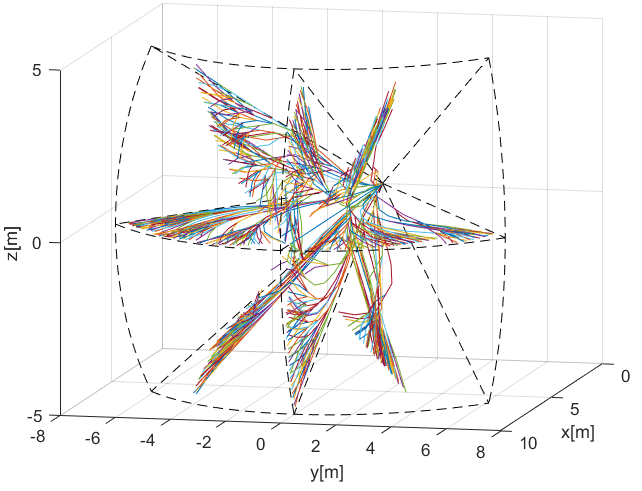
\includegraphics[width=0.9\linewidth]{\FIGDIR/RS005ACASLikeReachSetEstimationMethodFull}
        \caption{Full.}
        \label{fig:acasLikeReachSetFull}
    \end{subfigure}
    \begin{subfigure}{0.48\textwidth}
        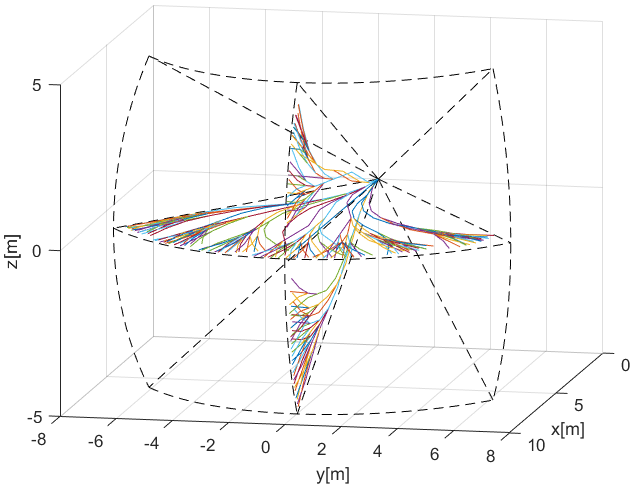
\includegraphics[width=0.9\linewidth]{\FIGDIR/RS006ACASLikeReachSetEstimationMethodHorizontalVertical} 
        \caption{Horizontal-Vertical.}
        \label{fig:acasLikeReachSetHorizontalVertical}
    \end{subfigure}
    \\
    \begin{subfigure}{0.48\textwidth}
        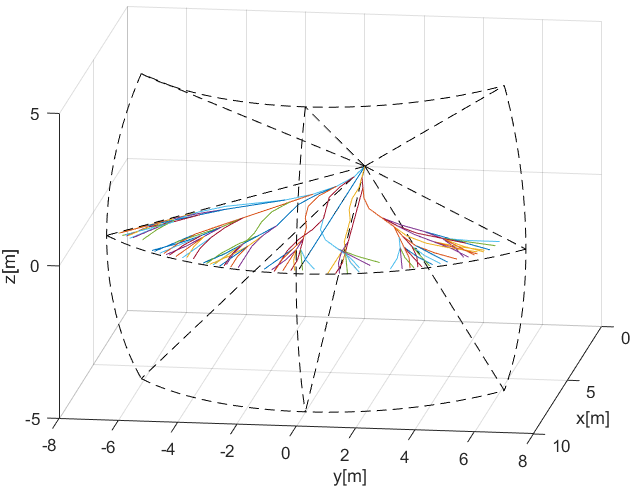
\includegraphics[width=0.9\linewidth]{\FIGDIR/RS008ACASLikeReachSetEstimationMethodHorizontal} 
        \caption{Horizontal.}
        \label{fig:acasLikeReachSetHorizontalOnly}
    \end{subfigure}
    \begin{subfigure}{0.48\textwidth}
        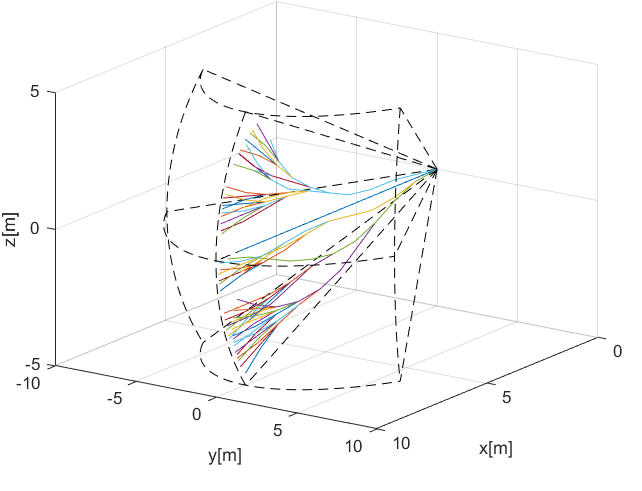
\includegraphics[width=0.9\linewidth]{\FIGDIR/RS009CASLikeReachSetEstimationMethodVertical} 
        \caption{Vertical.}
        \label{fig:acasLikeReachSetVerticalOnly}
    \end{subfigure}
    \caption{ACAS-X imitation \emph{reach set} approximation for various \emph{separation modes}. }
    \label{fig:acasLikeReachSetVariousSeparationMode}
\end{figure}

\paragraph{Pros and Cons:} It can be seen from examples (fig. \ref{fig:acasLikeReachSetVariousSeparationMode}) that \emph{ACAS-like Reach Set Approximation Method} (alg. \ref{alg:ExpansionConstraintFunctionForACASLikeReachSet}) generates full reach set for 2D plane located in 3D space. 

The \emph{Reach Set} contains trajectories with \emph{high coverage ratio} and \emph{high smoothness rating} for selected 2D separation plane. Overall performance compared to full 3D reach sets (sec. \ref{s:chaoticReachSet}, \ref{s:harmonicReachSet} \ref{s:combinedReachSet}) is poor. 

The \emph{node} and \emph{trajectory} count boundary was not implemented. It is common knowledge that \emph{2D} avoidance sets does not require scaling \cite{marston2015acas}. Otherwise trajectory footprint mechanism like in \emph{Harmonic Reach Set Approximation} (alg. \ref{alg:ExpansionConstraintFunctionForHarmonicReachSet}) can be introduced.

This reach set implements \emph{Planar-Separation} as native feature, it can be used for both \emph{navigation} and \emph{avoidance} tasks in \emph{Controlled Airspace}. For \emph{Non-controlled Airspace} there are far more superior \emph{Combined Reach Set} (sec. \ref{s:combinedReachSet}).

	

    %Observations moved to Conclusion - no longer in use
    %\section{(W) Simulation Observations Summary}\label{sec:SimulationObservationsSummary}
    \noindent Use summary of this section in Conclusion and future work on specific 

\subsection{(W) Static Obstacles Avoidance}\label{sec:staticObstacleAvoidanceSummary}
    \noindent TODO: main points of building, slalom, maze scenarios - link artifacts and performance criteria

\subsection{(W) Constraints Avoidance}\label{sec:constraintAvoidanceSummary}
    \noindent TODO constraints main point, main loop processing, breach chance ? etc...
    
\subsection{(W) Unsupervised Intruder Avoidance}\label{sec:unsupervisedIntruderAvoidance}
    \noindent TODO emergency intruder avoidance emphasis navigation, Emergency avoidance contribution main points

\subsection{(W) Supervised (UTM) Intruder Avoidance}\label{sec:supervisedIntruderAvoidance}
    \noindent TODO UTM contribution main points
    
 

%% This adds a line for the Bibliography in the Table of Contents.
\addcontentsline{toc}{chapter}{Bibliography}
%% *** Set the bibliography style. ***
%% (change according to your preference/requirements)
%\bibliographystyle{plain}
%% *** Set the bibliography file. ***
%% ("thesis.bib" by default; change as needed)
\bibliography{thesis}

%% *** NOTE ***
%% If you don't use bibliography files, comment out the previous line
%% and use \begin{thebibliography}...\end{thebibliography}.  (In that
%% case, you should probably put the bibliography in a separate file and
%% `\include' or `\input' it here).

\end{document}
